\chapter{Data Analysis}
This chapter presents two applications of Bayesian data analysis to different parts of the calorimetric $^{163}$Ho spectrum measured
by Holmes. A preliminary section provides a brief description the data processing techniques used to obtain a
calibrated energy spectrum from the raw signals, and of the expected background. The first part of the
analysis focuses on the M1 peak, using experimental data from 16 detectors. A basic
model is established and then expanded in order to describe an eventual asymmetry of the peak and fit all the available
data simultaneously, providing a preliminary measurement of the M1 position and width. The second part estimates a
plausible upper limit on the neutrino mass that could be achieved by Holmes in the near future, focusing on prior
sensitivity analysis and providing robust estimates from simulations of a low-activity measurement campaing. The chapter
concludes with a simulation of data from 64 different detectors, showing that for the low available statistics and under
the assumption that the systematics of the detectors are distributed normally a simple fitting procedure can be
applied to obtain consistent results.
\section{Preliminary considerations}
\subsection{Data elaboration}
As outlined in Section \ref{sec:muMUX}, the signals from the Transition Edge Sensors are observed as phase changes in the circuit's response to a certain microwave frequency. The raw signals are acquired through a time derivative trigger, resulting in a collection of pulses with the same length. To obtain a well-calibrated energy spectrum, the raw data must be carefully processed and corrected for the non-ideal behavior of the detectors. This data elaboration phase involves several distinct steps, which are briefly presented here.

\subsubsection*{Preanalysis}
The basic informations extracted from each raw signal include its baseline, given by the pre-trigger samples, the raw
amplitude, the rise time $RT$, and the decay time $RD$. In the initial stage of data elaboration, these quantities are
used to categorize the signals into six distinct types based on their pulse shapes. These categories, determined through
a series of filtering operations with adjustable threshold parameters, are crucial for the rest of the processing:

\begin{description}
\item[Empty:] Events containing noise.
\item[Strange:] Events exhibiting shapes differing from what is expected. 
\item[Bad:] Signals rising on the tail of a previous pulse, for which accurate energy identification is challenging due to the TES non-linearity.
\item[Multiple event:] Pile-up pulses rising from the tail of a triggered signal.
\item[Coincidence:] Muons or natural radioactivity background interacting with multiple detectors at the same time.
\item[Good:] All events not falling into the previous categories.
\end{description}

\subsubsection*{Optimum Filter}
The optimum filter is employed to refine the raw signal amplitude into another estimator more suitable for energy
calibration. This method allows the construction and application of a frequency filter to the signal, theoretically
maximizing the signal-to-noise ratio under specific assumptions. Each sample $s_i$ of a pulse is considered to be a
linear combination of a constant factor $K$ related to energy, a noise component $n_i$, and an underlying medium pulse $m_i$, as in $s_i = K m_i + n_i$. Given an ergodic noise with power spectral density $N$ and a signal sampled at a sufficiently high rate, the optimum filter $H$ is constructed from the Discrete Fourier Transform (DFT) of the samples $S$ and of the mean pulse $M$:
\begin{eqnarray}
 H_i \propto \frac{M_i^*}{N_i}\\
s^{OF}_i = \text{DFT}^{-1}(H \cdot S)_i
\end{eqnarray}
In this case, $N$ is computed from the average DFT of the signals tagged as "empty," which contain noise, while the mean pulse is obtained from a series of "good" events corrected for their arrival time. The resulting filtered "good" signals and their amplitudes are used as the basis for the following elaborations.

\subsubsection*{Gain Drift Correction}
Detector gain and baseline fluctuate over time due to temperature and voltage variations, leading to different signal
amplitudes for the same energy deposition. This gain drift also leads to a correlation between signal amplitude and
baseline, which can often be approximated as linear or quadratic due to the fluctuations being small. This allows
correcting the gain drift by removing the correlation between these two quantities. Events within a mono-energetic peak are fitted with a low-order polynomial in the amplitude/baseline plane, and all data are corrected following the fit results.

However, this process is complicated by the sudden signal jumps that can be attributed to fluctuations in the number of
Phase Slip Lines, as detailed in Section \ref{sec:TES}. As shown in Fig. \ref{fig:drift}, events in these time
intervals feature a different slope between amplitude and baseline, and must be removed from the dataset since they
cannot be corrected properly. 

At this stage, the data is represented as an n-tuple associating each signal with a series
of parameters, such as its time of recording, raw amplitude, OF amplitude, rise-time, and decay-time. This allows
filtering events by selecting intervals of these parameters. The selected regions can be intersected or added, globally
constituting what is known as a cut. For the scope of drift correction, it is then necessary to perform a series of cuts
on the timestamps to select only events with the same correlation between amplitude and baseline. An algorithm utilizing
reinforcement learning is under development to automate this selection procedure.

To correct the gain drift simultaneously across the entire acquired energy range, the latter is divided into small regions where the coefficients of the correcting polynomial can be considered constant. The actual fit and removal of the correlation are carried out in the intervals containing the peaks from calibration sources or from $^{163}$Ho. The results are then extrapolated to the other regions of the spectrum using a spline.

\begin{figure}[t]
  \centering
  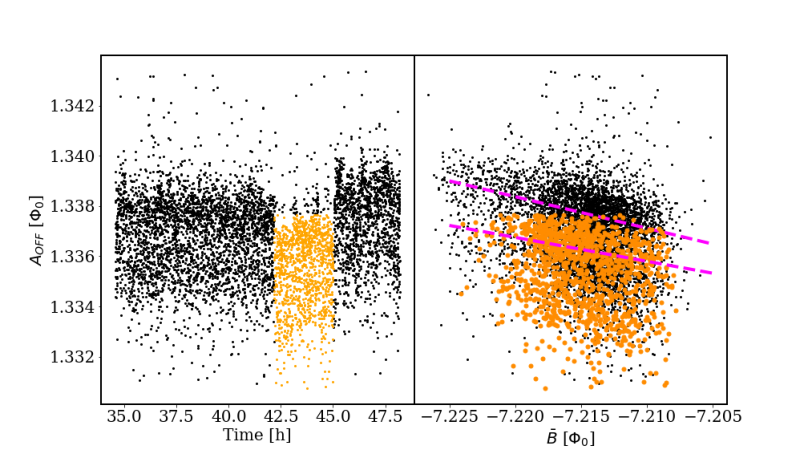
\includegraphics[width=0.77\textwidth]{figures/ch3/drift.pdf}
  \caption{Effect of sudden jumps in the detector response on the gain drift correction. Events in the corresponding
  time interval feature a different correlation between amplitude and baseline. Image taken from
\cite{borghesi2022toward}.}
  \label{fig:drift}
\end{figure}

\subsubsection*{Energy Calibration}
Leveraging the X-ray sources described in Section \ref{sec:holder}, the energy response of each detector is
calibrated using the processed signals obtained after applying the optimum filter and correcting the gain drift.
Calibration is performed by fitting some known X-ray peaks originating from the calibration source with one or more Gaussians. The peak energies $E_{OF}$ obtained
from the fit can be compared with the true known energies of the decays $E_{true}$. The calibration curve $E_{OF}
(E_{true})$ is then given by a low-order polynomial or a spline interpolating the points computed by fitting each peak. For the calibration of the data used in this thesis, a spline was employed.

The accuracy of the procedures leading to a calibrated spectrum can be verified by comparing the estimate of the energy
resolution $\Delta E$ obtained from the fit of a known X-ray peak, typically the $K_\alpha$ line of $^{55}$Mn, with that
given by the Noise Equivalent Power (NEP). The NEP determines $\Delta E$ from the noise power spectrum and the
detector's responsivity, assuming a delta signal for energy deposition, and can be considered as a lower bound for the
energy resolution reachable after calibration.

Achieving precise calibration is vital for characterizing the $^{163}$Ho spectrum, particularly in exploratory runs
aiming to characterize the decay spectrum by determining the parameters of the main Lorentzian peaks and measure the
$Q$-value. The calibration systematics will play a central role in the construction of the fit models used in this chapter.

\subsection{Expected Background and Background Rejection}\label{sec:expected}
For the Holmes experiment, background can be considered to originate from either pile-up events or natural radiation and
cosmic rays. While the former is predicted to be predominant for detectors with high activity rates ($A > 50$ Bq), the
latter constitutes the main source of background in a low-activity measurement. Pileup and radioactivity are predicted to
contribute similarly to the background for intermediate activities ($A \sim 10$ Bq).

To assess the natural radioactivity background, preliminary measurements were conducted without any kind of calibration
source or Holmium in the detectors \cite{borghesi2022toward}. The resulting background signals were separated into events involving multiple TESs
at the same time or a single TES. Due to the dimensions of the absorbers compared to the rest of the array, the TES-TES
coincidences are the most probable, generated by radiation interacting with the material between the pixels. At the same
time, many of the single TES background events consist of radiation directly hitting a thermometer or its surroundings
instead of the corresponding absorber. Both of these processes lead to signals that are significantly
different from those originated from $^{163}$Ho implanted in the absorbers and can be identified through their rise time
and decay time. This allows for the suppression of the background rate through cuts on these parameters, selecting only
the events that interact directly with a single absorber. 

In the characterization run, this method reduced the
background rate from $0.5 \times 10^{-3}$ counts eV$^{-1}$day$^{-1}$det$^{-1}$ to $1 \times 10^{-4}$ counts eV$^{-1}$day$^{-1}$det$^{-1}$ in the region around the endpoint, which is denoted as the Region of Interest (ROI) for neutrino
mass searches. Moreover, the characterization measurements showed that the background is practically flat in the regions
containing the M peaks and the endpoint. It is estimated that almost half of the background events are originated from muons, which could be further suppressed by applying a coincidence veto.

\begin{figure}[t]
  \centering
  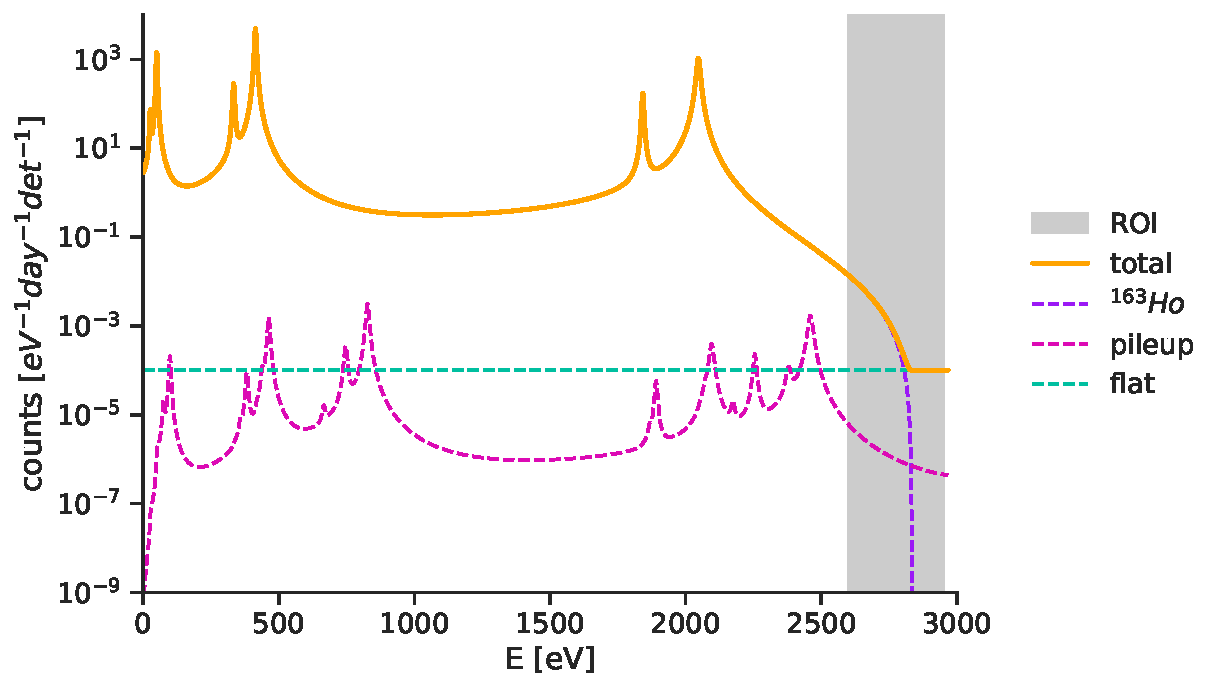
\includegraphics[width=0.85\textwidth]{figures/ch3/spectrum_0.pdf}
  \caption{First-order spectrum with expected flat background and pileup.}
  \label{fig:expected}
\end{figure}
The expected pileup for a certain detector can instead be computed considering its time resolution $\tau_R$ and activity
$A$, with a rough estimate being given by $f_{pp} = \tau_RA$. This estimate can be improved by also considering the pulse
length $L$. Given an energy ROI$=[E_{min}, E_{max}]$, the expected fraction of pileup $f_{pp}$ is computed from 
the probability of events containing a single pulse $P_s$ and that of events containing an additional pulse in
the first $\tau_R$ microseconds from the beginning of the signal ($P_{d}$). The probabilities are weighted by the
integral
of the spectrum and pileup spectrum in the ROI:
\begin{eqnarray}
f_{pp} &=& \frac{P_d}{P_s}\\
P_d &=& \text{Poisson}(1 \mid \tau_R \times A) \int_{E_{min}}^{E_{max}} S(E) * S(E) dE\\
P_s &=& \text{Poisson}(0 \mid L \times A) \int_{E_{min}}^{E_{max}} S(E) dE
\end{eqnarray}
While without further elaboration the time resolution coincides with the sampling time of the signal, with the
application of filtering techniques and cuts it is possible to reduce it by a factor of two. For the current
configuration $\tau_R = 2 \mu$s, while $L = 4$ ms. Considering an activity of $\sim 1$ Bq, this results in an expected
pileup fraction $f_{pp} \sim 2 \times 10^{-6}$ over the whole spectrum. The first-order spectrum with the expected
background is shown in Fig \ref{fig:expected}.



\section{Spectrum characterization}
\subsection{Acquired data}
This section presents the analysis of data obtained during a characterization run using a calibration source and the
experimental setup
described in Sec \ref{sec:setup}. The data was collected from the array implanted with a single central spot
of $^{163}$Ho. Out of the 64 detectors in the array, 54 provided consistent readings, while the others were discarded
due to various detector imperfections, such as defective resonators on the $\mu$MUX chip.

The resulting activity map, shown in Figure \ref{fig:data} (a), represents the event rate in each detector. While the
profile of the beam used for implanting the isotope doesn't appear to be gaussian, the higher activity at the center of
the array indicates proper alignment. However, the observed activity of $^{163}$Ho in the central detectors seems to be three times lower than expected.

Though the activity is too low to study the spectrum endpoint within a reasonable time, this setup is suitable for
characterizing the rest of the spectrum. Figure \ref{fig:data} (b) shows a spectrum obtained
by combining data from four detectors. Besides the four main peaks of the first-order spectrum, additional features can be
observed, such as second-order peaks after M1, and an asymmetric slope in the broad region between N1 and M2. The peak
at around 1500 eV corresponds to the K$_\alpha$ line of aluminum in the calibration source.

The observed energy resolution for all detectors ranges between 5 and 10 eV, with a mean NEP estimate of $7.3\pm 1.3$ eV. However, comparing the acquired spectra
reveals systematic effects introduced during the data processing, altering the measured energy in each detector, as
depicted in Figure \ref{fig:data} (c). While these systematics will require further investigation, in this thesis they
will be treated as an overall energy shift in each detector's response.

This analysis focuses on the M1 peak, which is of particular interest for neutrino mass estimation as it is the closest
to the endpoint. The Region of Interest is chosen to be between 1950 eV and 2150 eV. Only data from the 16 detectors
with the highest activity is considered, resulting in approximately 161,000 events in the ROI, with each detector having
measured between 1600 and 25,500 pulses.

Considering both natural radioactivity and pileup, the total fraction of background events in the ROI is expected to
be around $10^{-6}$ for the detector with the highest activity and approximately $1.5 \times 10^{-5}$ for the detector
with the lowest. Since the expected number of background events in each detector is less than one, background effects
can be safely neglected in the following analysis.

\begin{figure}[t]
\begin{subfigure}[b]{0.45\linewidth}
  \hfill
  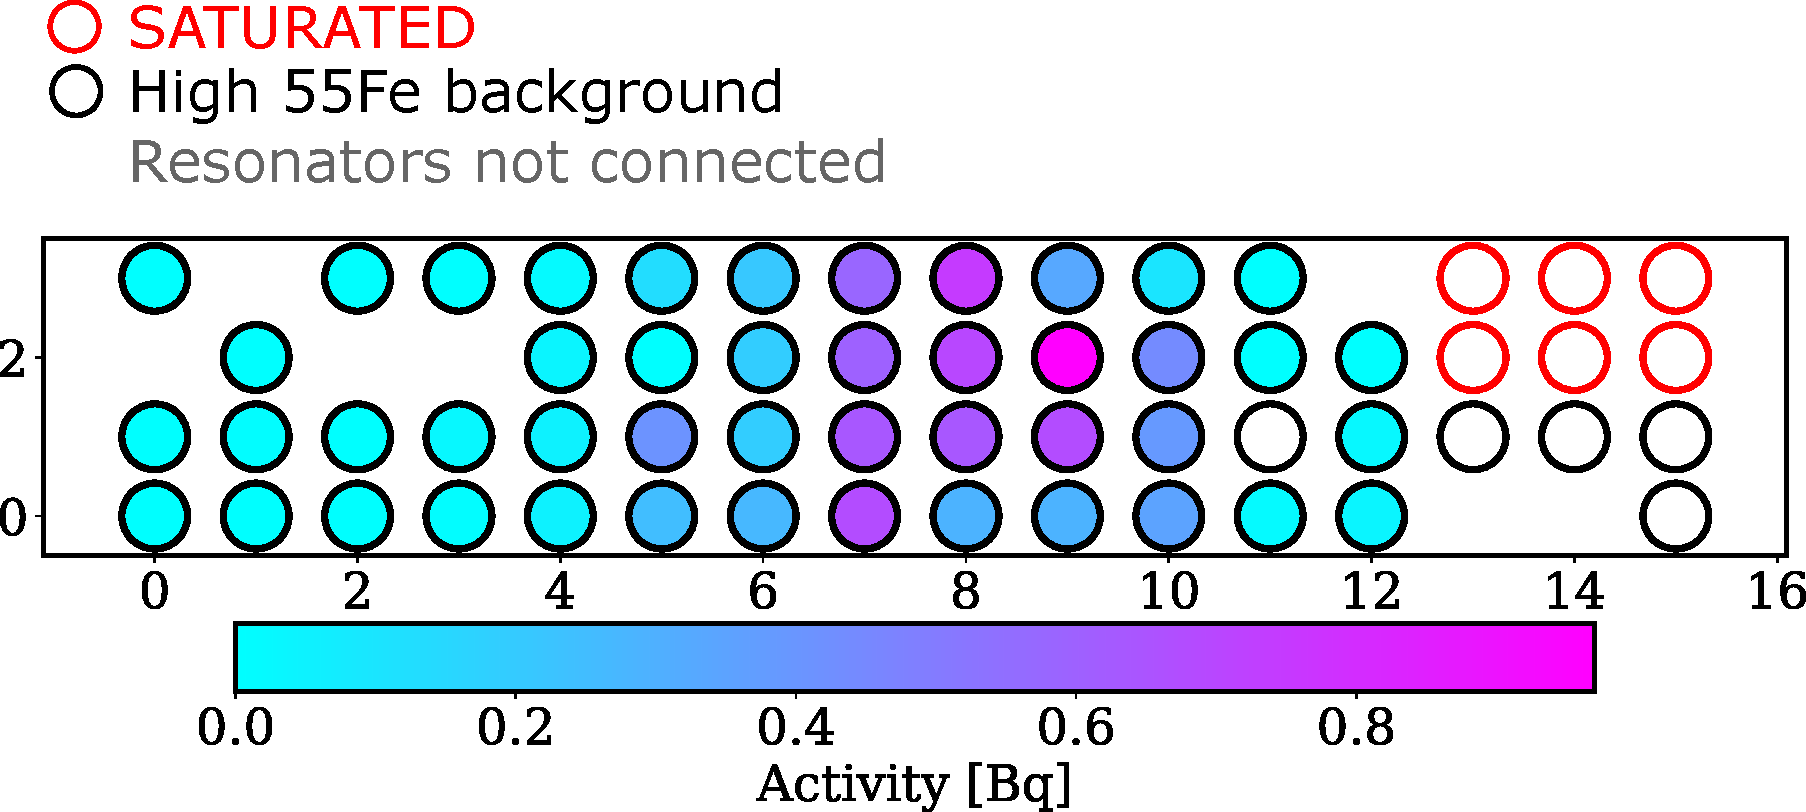
\includegraphics[width=\linewidth]{figures/ch3/activity_tesA.pdf}
  \hfill
  \caption{}
\end{subfigure}
\begin{subfigure}[b]{0.55\linewidth}
  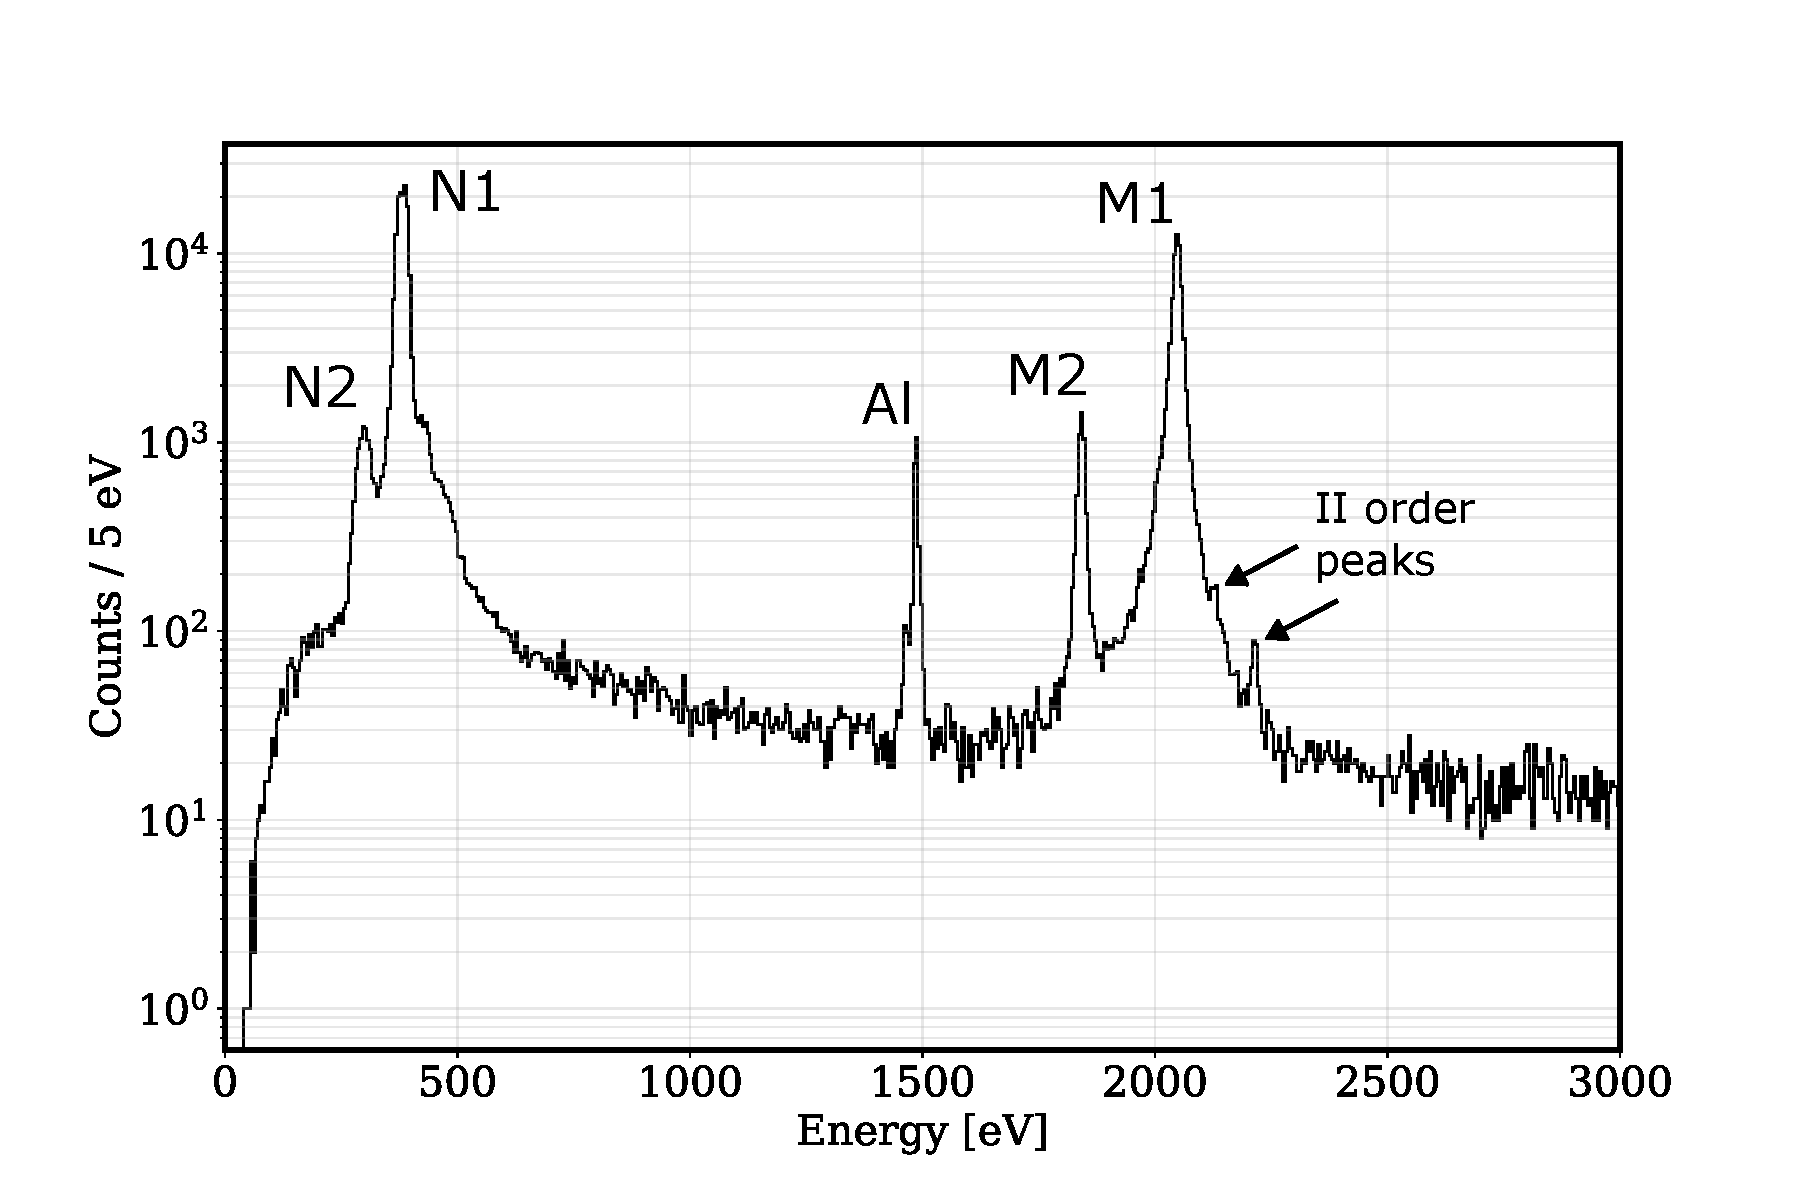
\includegraphics[width=\linewidth]{figures/ch3/Ho_combined.pdf}
  \caption{}
\end{subfigure}
\begin{minipage}{\textwidth}
\begin{subfigure}[b]{\linewidth}
  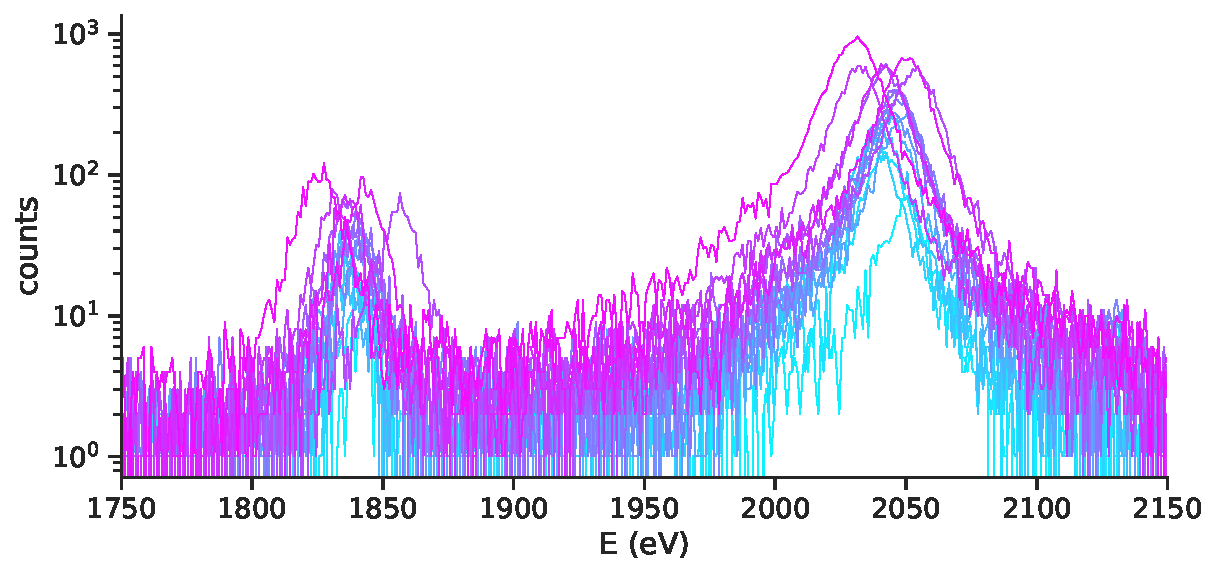
\includegraphics[width=\linewidth]{figures/ch3/peaks/M1M2_0.pdf}
  \caption{} 
\end{subfigure}
\end{minipage}
\caption{Activity map of the 64 TES array in the initial measurement of Holmes (a). First acquired $^{163}$Ho spectrum obtained by
combining data from 4 TESs (b). Focus on the M1 and M2 region of the spectrum acquired by the 16 detectors with the
highest activity. Systematics in the energy calibration shift the observed spectrum differently for each detector (c).}
\label{fig:data}
\end{figure}


\subsection{Single detector model}
To begin, a single detector is considered and approximate function is used to fit the observed M1 peak, with the aim to
characterize its main parameters: the position $E_{M 1}$ and width $\Gamma_{M 1}$.
The underlying peak is therefore described by a Lorentzian summed to a first-order polynomial, which approximates the
other features in the spectrum, multiplied by the phase space of Eq \ref{eq:hofirstorder}:

\begin{equation}
  S(E)= [L(E, E_{M 1}, \Gamma_{M 1}) + m(E-E_0) + y_0)]\times PS(E, Q, m_\nu)
\end{equation}

In this equation, $L$ is the Lorentzian representing the M1 peak, while the polynomial is constructed relative to the initial point $E_0$ of the
ROI. For the phase-space term $PS$, a neutrino mass of 0 eV and  $Q=2833$ eV will be assumed in the following
analysis. To obtain the experimental spectrum $S_{\exp}(E)$, $S(E)$ is convolved with a gaussian function of width
$FWHM$ representing the resolution of the detector. The resulting spectrum is normalized to 1 in the ROI.

The basic model used for this fit includes the following free parameters: the peak position $E_{M1}$, its width $\Gamma_{M1}$, the
intercept $y_0$ and slope $m$ of the polynomial, the
energy resolution of the detector $FWHM$, and an overall normalization factor $A$ to account for fluctuations of the observed number of events $N_{tot}$ in the ROI. 
The fit is performed by binning the data with a bin width of 1 eV and assuming Poisson fluctuations for the number of
events $N_{ev}[i]$ in each bin. The convolution operation between the theoretical spectrum and the Gaussian experimental
response is handled carefully to avoid border effects. The spectrum is initially computed over a wider range, determined
by the width of the Gaussian response, and then trimmed down to the ROI. Additionally, a convolution function using the
Fast Fourier Transform (FFT) is implemented in Stan to improve efficiency.


The model's priors constrain the parameters within their expected ranges. The resonance position $E_{M1}$ follows a
weakly regularizing prior given by a normal distribution centered on the expected value from the first-order approximation
($E_{M1}^{th} = 2047$ eV) and with a standard deviation of 50 eV. Similarly, $\Gamma$ has a Gamma prior centered on 13.2 eV,
with 90\% of the probability mass between 5 and 25 eV. The prior for $FWHM$ considers the estimate given by the NEP as
a lower bound. Since the NEP is usually obtained with $\pm 0.2$ eV precision, the Frechet distribution is used to construct a prior with 99\% of the probability falling between $NEP-0.4$ eV and $NEP+4$ eV. The normalization factor $A$ is
considered to vary around 1 with a normal standard deviation of 0.05. Finally, the intercept and slope of the polynomial are
given very tight normal priors in order to prevent the overall spectrum from becoming negative in some points:
\begin{figure}[t]
\begin{subfigure}[b]{0.45\linewidth}
    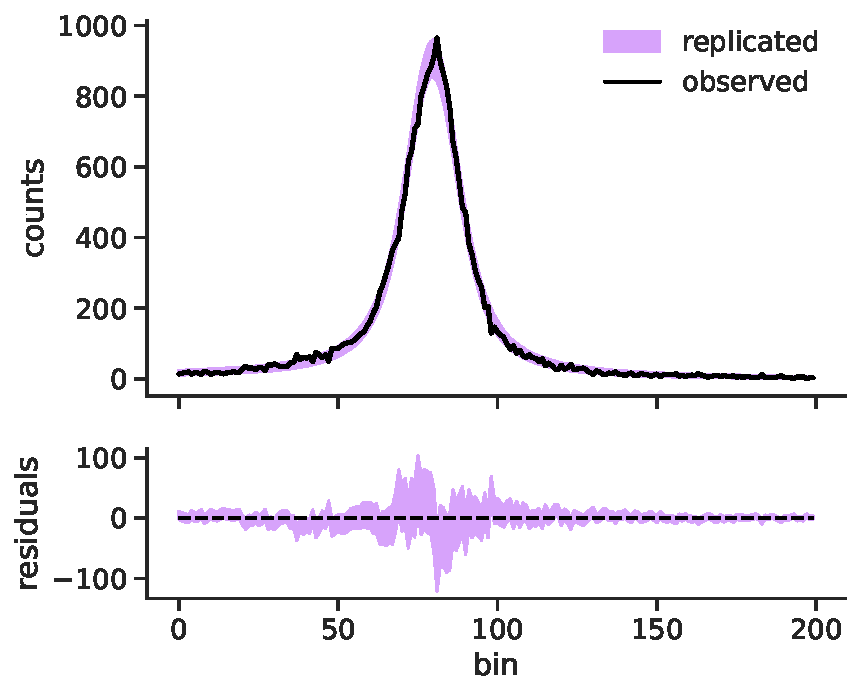
\includegraphics[width=\linewidth]{figures/ch3/peaks/predictive_check_1.pdf}
\caption{}
\end{subfigure}
\hfill
    \begin{subfigure}[b]{0.45\linewidth}
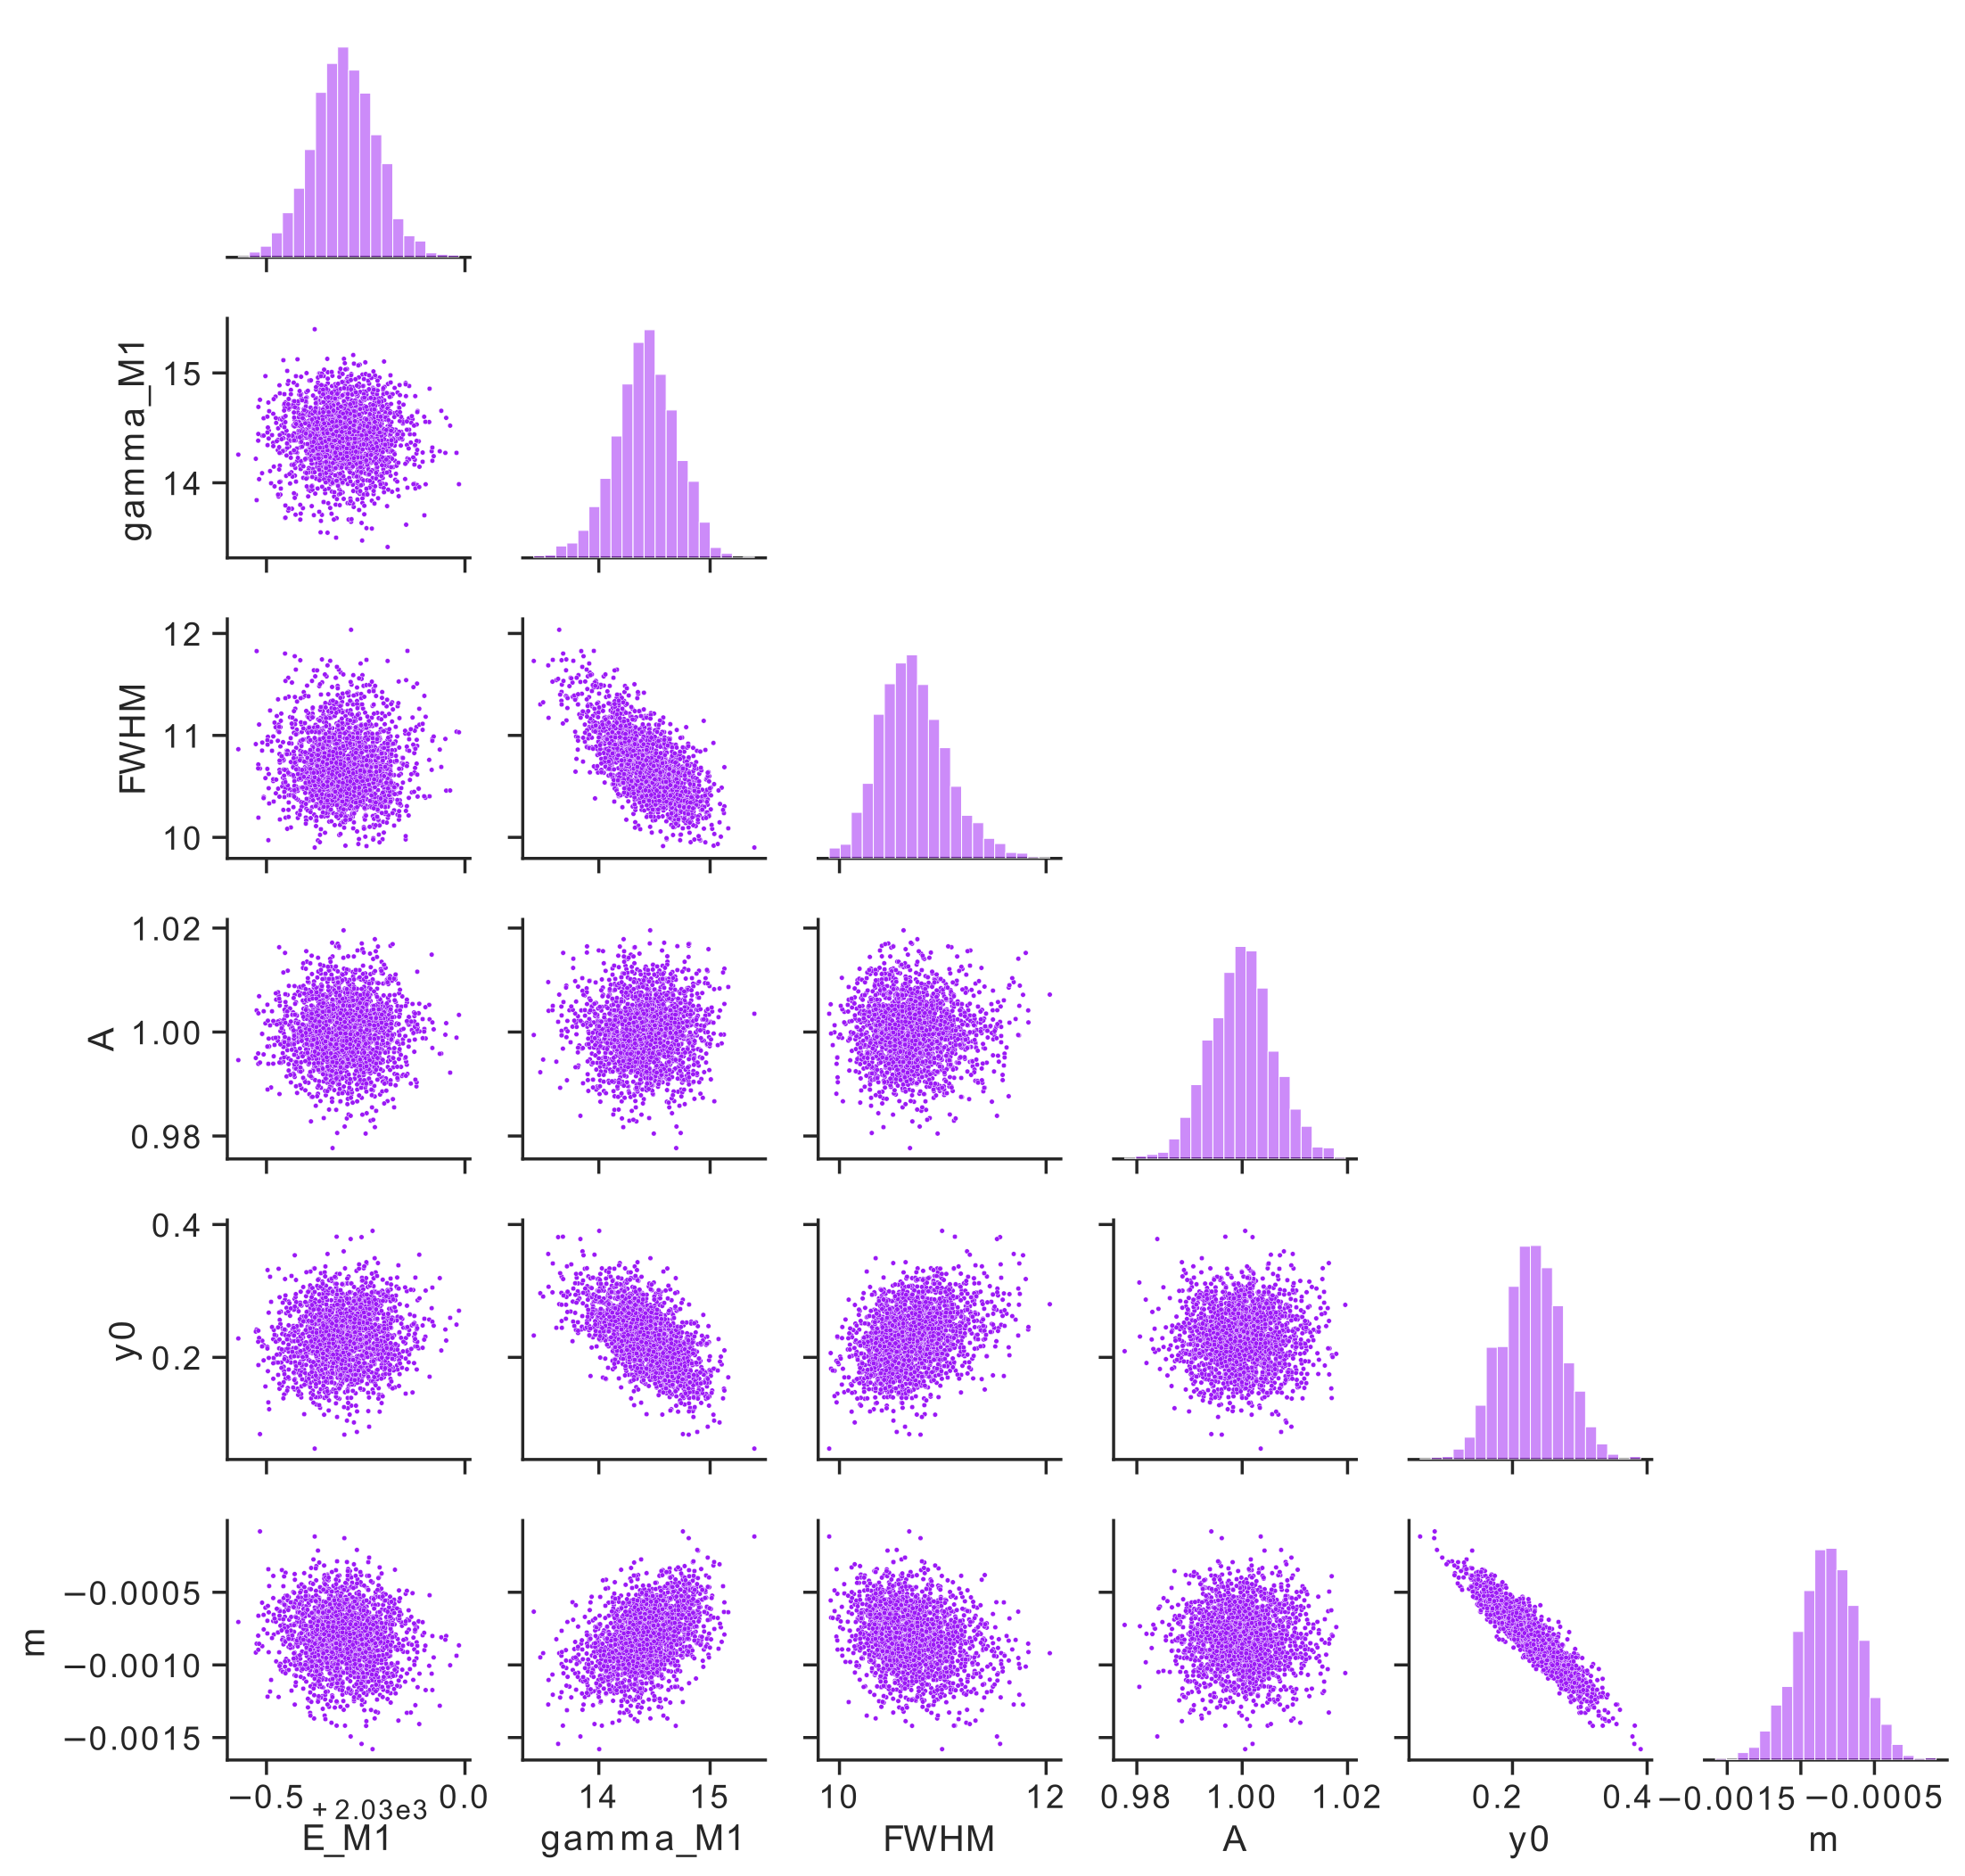
\includegraphics[width=\linewidth]{figures/ch3/peaks/pair_grid_0.png}
\caption{}
\end{subfigure}
\caption{Posterior predictive check for the simple M1 peak model, note the asimmetry of the residuals around the peak (a). Correlations between parameters in the posterior of
the model (b). Data taken from the detector with highest statistics, corresponding to 25500 events in the ROI and
$FWHM=10.5$ eV.} 
\label{fig:peakcorr}
\end{figure}
\begin{eqnarray}
  E_{M 1} &\sim& \text{normal}(2047, 50)\\
  \Gamma_{M 1} &\sim& \text{gamma}(6.6, 0.5)\\
  y_0 &\sim& \text{normal}(0,0.02)\\
  m &\sim& \text{normal}(0,0.01)\\
  FWHM &\sim& \text{frechet}(2\times NEP, \;NEP+0.5)\\
  A&\sim& \text{normal}(1, 0.05)\\
  N_{ev}&\sim& \text{poisson}(S_{\exp}(E, E_{M 1}, \Gamma_{M 1}, y_0, m, FWHM)\times A\times N_{tot})
\end{eqnarray}





The model is efficient, completing the warm-up phase and generating 1000 samples from each Markov chain in less than 10
seconds. Stan's diagnostics do not raise any warnings regarding potential issues, and all the posteriors of the
parameters are narrower than their priors. Figure \ref{fig:peakcorr} presents the
posterior predictive check and correlations between the parameters. While some strong correlations are observed, they do
not introduce significant curvature in the posterior's geometry, and Stan appropriately accounts for them by adjusting
the HMC metric. However, the residuals in the posterior predictive check suggest that the model does not perfectly describe the data. Notably, the residuals appear mostly positive on one side of the peak and mostly negative on the other, possibly indicating a slight asymmetry.

\begin{figure}[t]
  \centering
  \begin{minipage}{0.45\linewidth}
    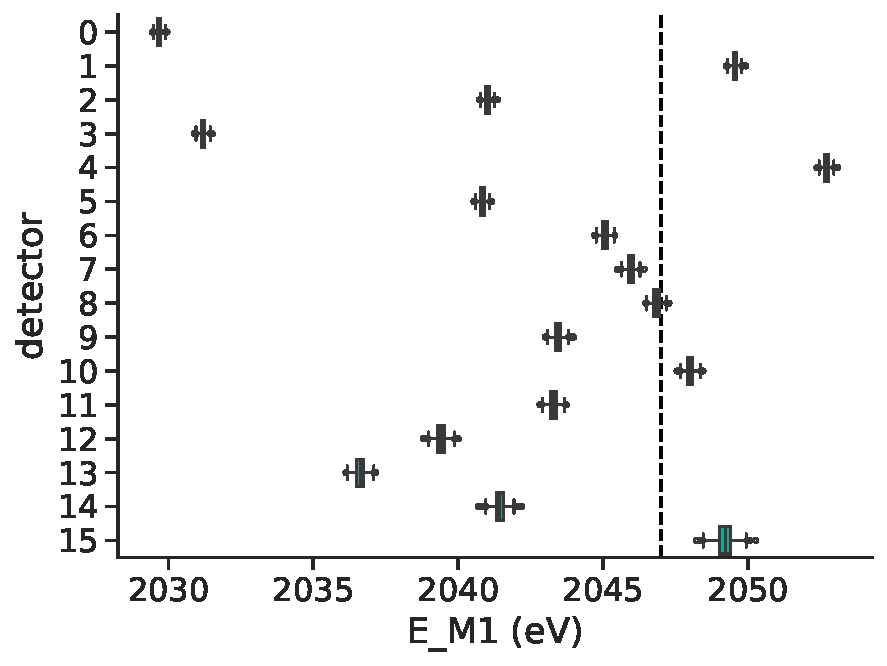
\includegraphics[width=\linewidth]{figures/ch3/peaks/cat_plot_0.pdf}
  \end{minipage}
  \centering
  \begin{minipage}{0.45\linewidth}
    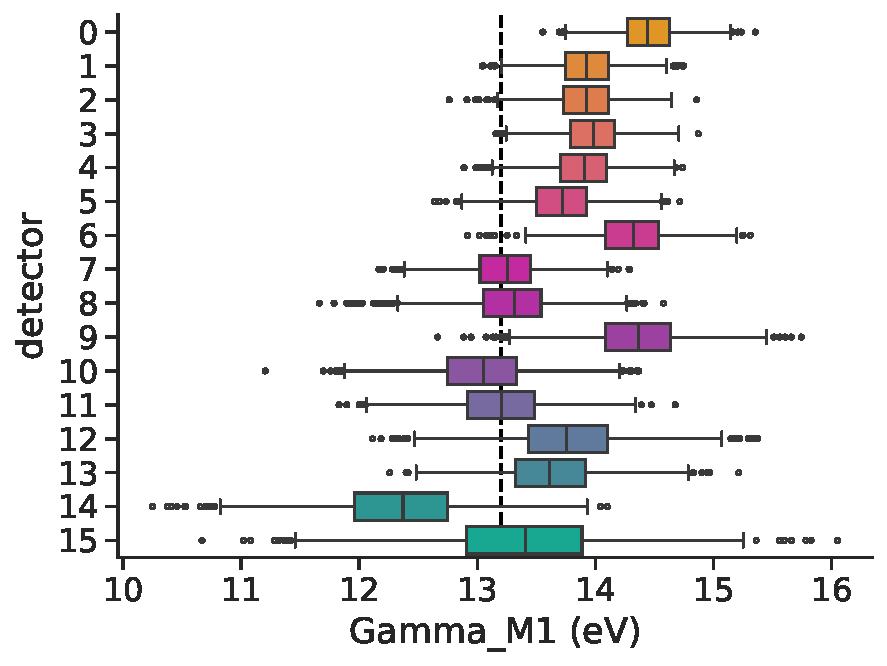
\includegraphics[width=\linewidth]{figures/ch3/peaks/cat_plot_1.pdf}
  \end{minipage}
 % \begin{minipage}{0.33\linewidth}
 %   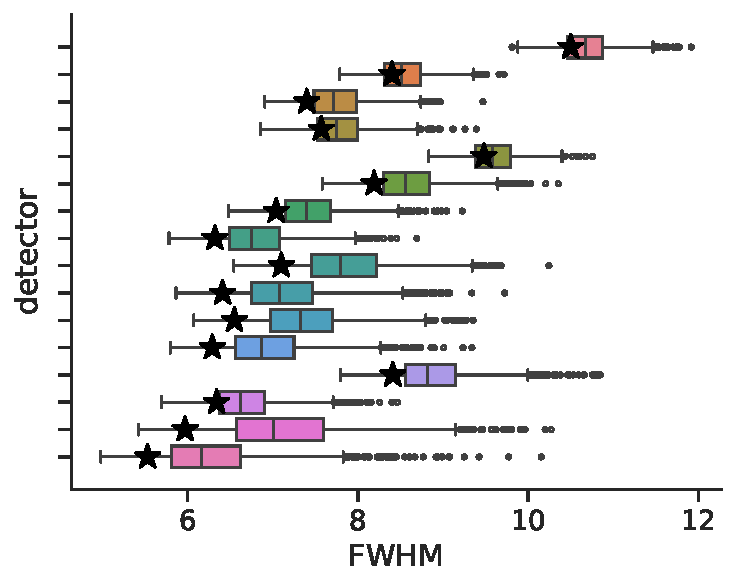
\includegraphics[width=\linewidth]{figures/ch3/peaks/cat_plot_2.pdf}
 % \end{minipage}
 % \hfill
 % \begin{minipage}{0.33\linewidth}
 %   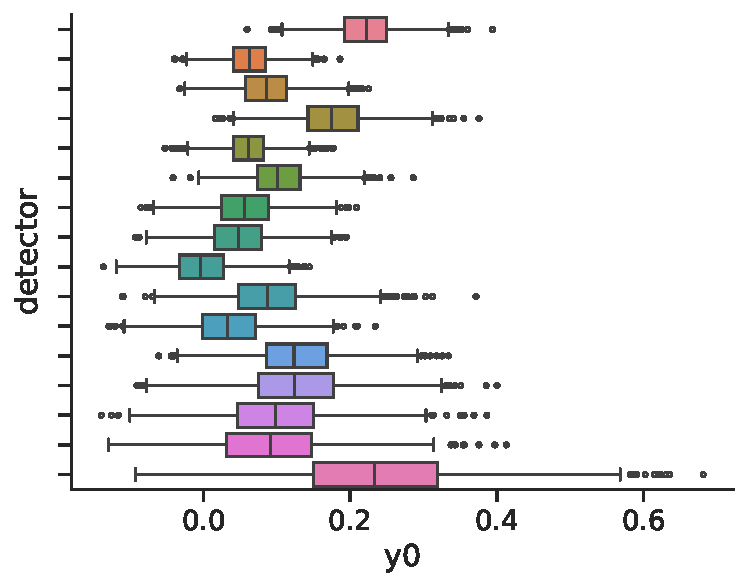
\includegraphics[width=\linewidth]{figures/ch3/peaks/cat_plot_4.pdf}
 % \end{minipage}
 % \begin{minipage}{0.33\linewidth}
 %   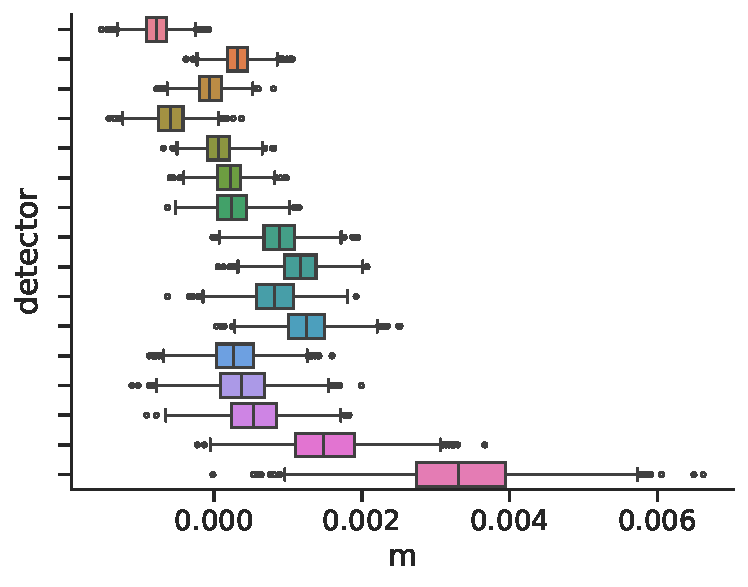
\includegraphics[width=\linewidth]{figures/ch3/peaks/cat_plot_5.pdf}
 % \end{minipage}
 % \begin{minipage}{0.33\linewidth}
 %   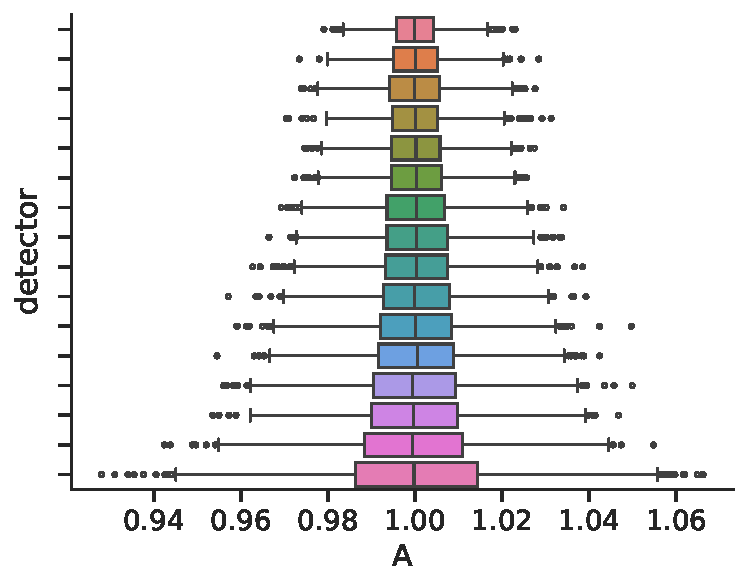
\includegraphics[width=\linewidth]{figures/ch3/peaks/cat_plot_3.pdf}
 % \end{minipage}
\caption{Posterior boxplots of independent fits of the M1 peak for 16 detectors, ordered by acquired statistics. The
black lines correspond to the first-order predictions}%, while the blackstars in the graph for $FWHM$ represent the expected energy resolution computed with the NEP.}
\label{fig:singlepeak}
\end{figure}
The fit has been independently repeated for all 16 considered detectors. The resulting posterior distributions for the two
parameters of the M1 peak
are shown in Figure \ref{fig:singlepeak}, with detectors ordered by acquired statistics, from highest (1) to
lowest (16). In each case, a value for $E_{M 1}$ identified with an accuracy of approximately 1 eV. However, due to the calibration
systematics this results in significantly different predictions for various detectors. On the other hand, results are more
consistent for the peak width, though they tend to be slightly higher than the first-order
prediction. The $FWHM$ of all detectors are found to be not more than 1 eV higher than the NEP estimate. A slightly positive slope and intercept of the polynomial is found in most cases,
while the normalization factor $A$ is tightly constrained around 1 due to the
relatively high statistics. 

\subsection{Lineshape asymmetry}
Higher order predictions introduce additional peaks in the spectrum and reveal an asymmetric broadening of resonances caused by Auger-Meitner decays. The latter phenomenon
involves the transfer of energy from an electron filling a vacant orbital created in the EC decay to
another electron, which is ejected from the atom into the continuum, contributing to what is known as the shake-off spectrum. These predictions, along with the observed
deviations in the residuals of the posterior predictive checks, highlight the need to model the M1 peak differently, taking into account a possible asymmetry due to unresolved additional peaks and shake-off.

%In previous studies using data from Echo, it was found that the broadening of the spectrum is consistent with a Mahan lineshape. While this approach is theoretically motivated, it is computationally demanding. Given that the rest of the spectrum is already approximated at the first-order, it is more practical to explore alternative descriptive models with lower computational overhead.

The first model, which will be denoted as LR asymmetry, constructs an asymmetric profile by combining two Lorentzian
distributions with different widths on either side of $E_{M1}$. These widths are defined as $\Gamma_L = (1-a)\Gamma_{M1}
$ and $\Gamma_R = (1+a)\Gamma_{M1}$, where $a$ represents the asymmetry parameter:
\begin{equation}
\text{Lorentzian}_{LR} \propto
\begin{cases}
L(E, E_{M1}, \Gamma_R) \quad \text{for} \quad E \geq E_{M1} \\
L(E, E_{M1}, \Gamma_L) \quad \text{for} \quad E < E_{M1}
\end{cases}
\end{equation}



\begin{figure}[t]
  \centering
  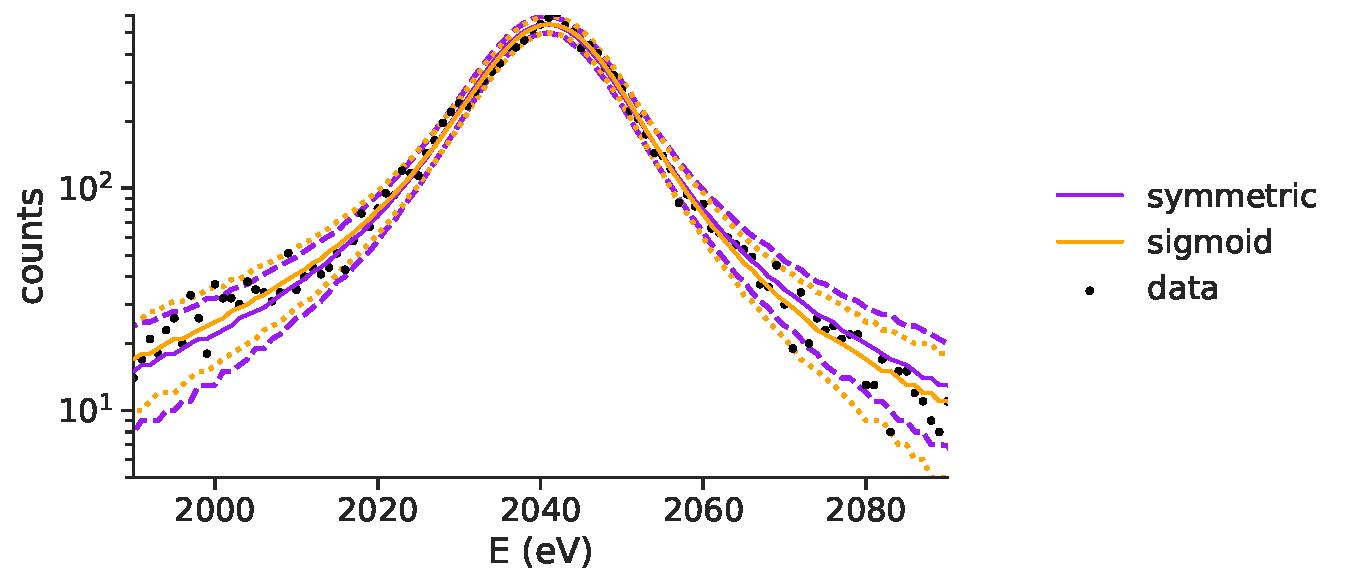
\includegraphics[width=0.87\textwidth]{figures/ch3/peaks/compred_0.pdf}
  \caption{Posterior predictive checks median and 95\% HDI comparing the symmetric and sigmoid width model with both $\alpha$
  and $\beta$. A slight asymmetry is visible in the tails of the M1 peak. Data taken from detector 5, corresponding to
15000 events in the ROI and $FWHM=7.5$ eV.}
  \label{fig:pred_asymm}
\end{figure}

Another approach to introduce asymmetry in the lineshape is to make the peak widths dependent on energy. Recent research \cite{schmid2014new} in characterizing X-ray photoelectric peaks has shown that using a sigmoid function to model the width accurately fits many experimental lineshapes. However, this introduces two additional parameters into the fit:
\begin{equation}
\Gamma_{M1} \rightarrow \Gamma(z, \Gamma_{M1}, \alpha, \beta) = \frac{2\Gamma_{M1}}{1+\exp(-\alpha(x-\beta))}
\end{equation}
Where $x = E - E_{M1}$. The parameter $\alpha$ controls the strenght of the asymmetry, while $\beta$ allows for
shifting from the center of the peak the point where the width changes. These new parameters
are added to the previous model with weak priors. Both $a$ for the LR and $\alpha$ for the sigmoid asymmetry model are limited to the
range of -0.5 to 0.5. For the second model, $\beta$ follows a normal distribution with a standard deviation of 15 eV, centered on 0 eV.
Both models converge without generating warnings. The predictive checks for the symmetric and the full sigmoid model are
shown in Figure \ref{fig:pred_asymm}. While significantly different results do not appear for all detectors, for some of
those with higher statistics the
posteriors for $\alpha$ are notably shifted away from 0, being centered around approximately $-0.01 \pm 0.003$. However,
the posterior for $\beta$ remains unchanged from the prior, even when broad priors are used.

This leads to consider whether to exclude the $\beta$ parameter from the sigmoid model to further reduce computational
overhead. Model comparison has been performed with Leave-One-Out Cross-Validation (LOOCV) to assess the predictive
performance of these three alternatives compared to the basic model with a symmetric Lorentzian. The resulting
estimates of the difference in expected log predictive density (elpd) from the symmetric profile are shown in Figure
\ref{fig:comp}.

In this case, the elpd difference is considered to allow visualizing the comparison across all detectors.
Additionally, the absolute elpd scores have relatively large standard errors, while the errors on the differences
are much smaller due to the absolute estimates being correlated.


\begin{figure}[t]
  \centering
  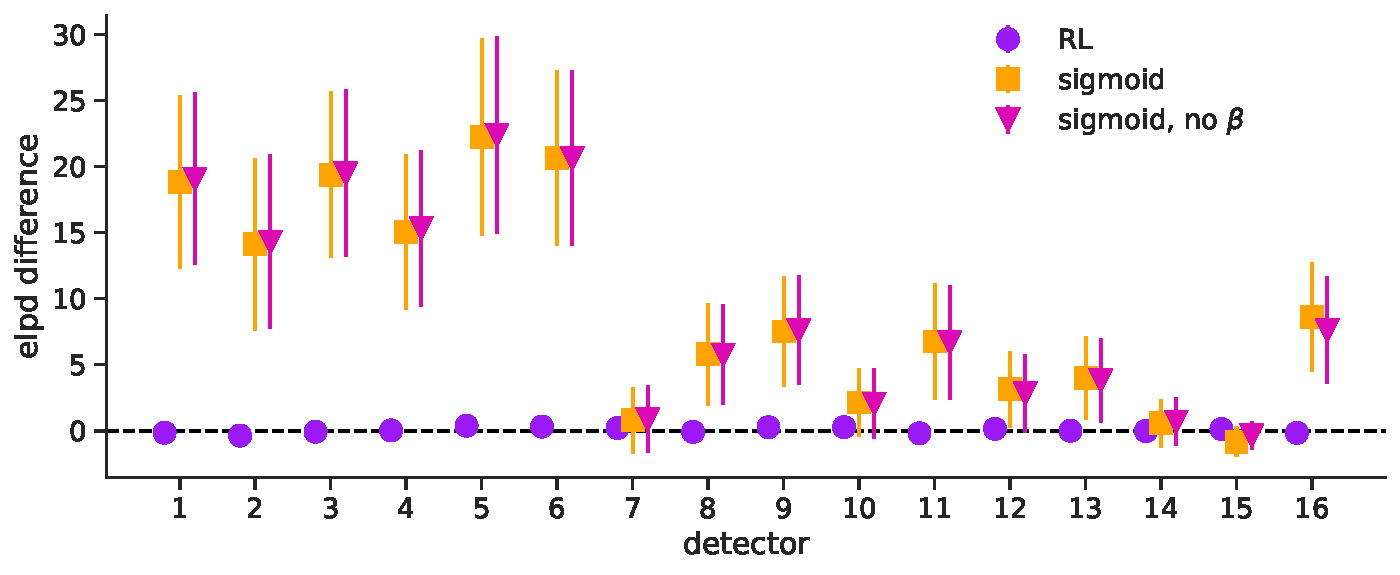
\includegraphics[width=0.75\textwidth]{figures/ch3/peaks/loooCV_0.pdf}
  \caption{Results of model comparison for different asymmetric lineshapes. The elpd difference with respect to the
  model without asimmetries is plotted on the y-axis for each detector. The two models with a sigmoid tend to
perform similarly, while the LR asymmetry model performs almost exaclty as the symmetric profile.}
  \label{fig:comp}
\end{figure}

In standard practice, an elpd difference above 4 can be considered significant if its error is sufficiently low. As
observed, most detectors benefit from the inclusion of the asymmetric profile. For the constructed estimates, the LR model is predicted to perform
almost exactly as the symmetric Lorentzian, with negligible errors, while both of those employing the sigmoid consistently reach higher and identical
elpd scores. Since the
elpd estimates for the model excluding the $\beta$ parameter and the one with both
$\beta$ and $\alpha$ are practically equivalent both in value and error, this leads
to the choice of using the sigmoid profile with only the additional parameter $\alpha$ to describe the shape of the M1
peak.



%, making the difference in predictive performance more significant. This illustrates how LOOCV and model comparison penalize overfitting,



\subsection{Multiple detectors and energy calibration systematics}
As shown in Fig. \ref{fig:singlepeak}, the energy calibration systematics do not allow obtaining compatible independent estimates of $E_{M 1}$ by
considering the detectors separately. In cases such as these, it is often uncertain how to combine the results.
For statistically compatible values it is usually adivised to do so with a weighted mean, considering the standard
deviation of each measurement, while for incompatible values it is otherwise suggested to compute the error on the overall
estimate as the standard deviation of the means. However, in this case the indipendent measurements of
$E_{M 1}$ are incompatible, but it is known that they actually belong to the same underlying parameter.




Instead of performing the fits separately and combining the results in an arbitrary way, it is possible to construct a single model that considers all the detectors
simultaneously and determines their energy calibration systematics and other parameters at the same time as $E _{M 1}$.
While $E_{M 1}$ and the calibration sistematics, denoted as $\delta E$, are clearly extremely correlated, it is still
possible to obtain sensible estimates of both by assuming that the values of $\delta E$ are distributed around zero.
Moreover, these additional parameters can be organized in a hierarchical prior, allowing to exchange information between
the detectors in their estimation. In this case, $\delta E$ is introduced as an overall shift of the energy read by
each detector.

\begin{figure}[t]
  \begin{minipage}{0.55\linewidth}
    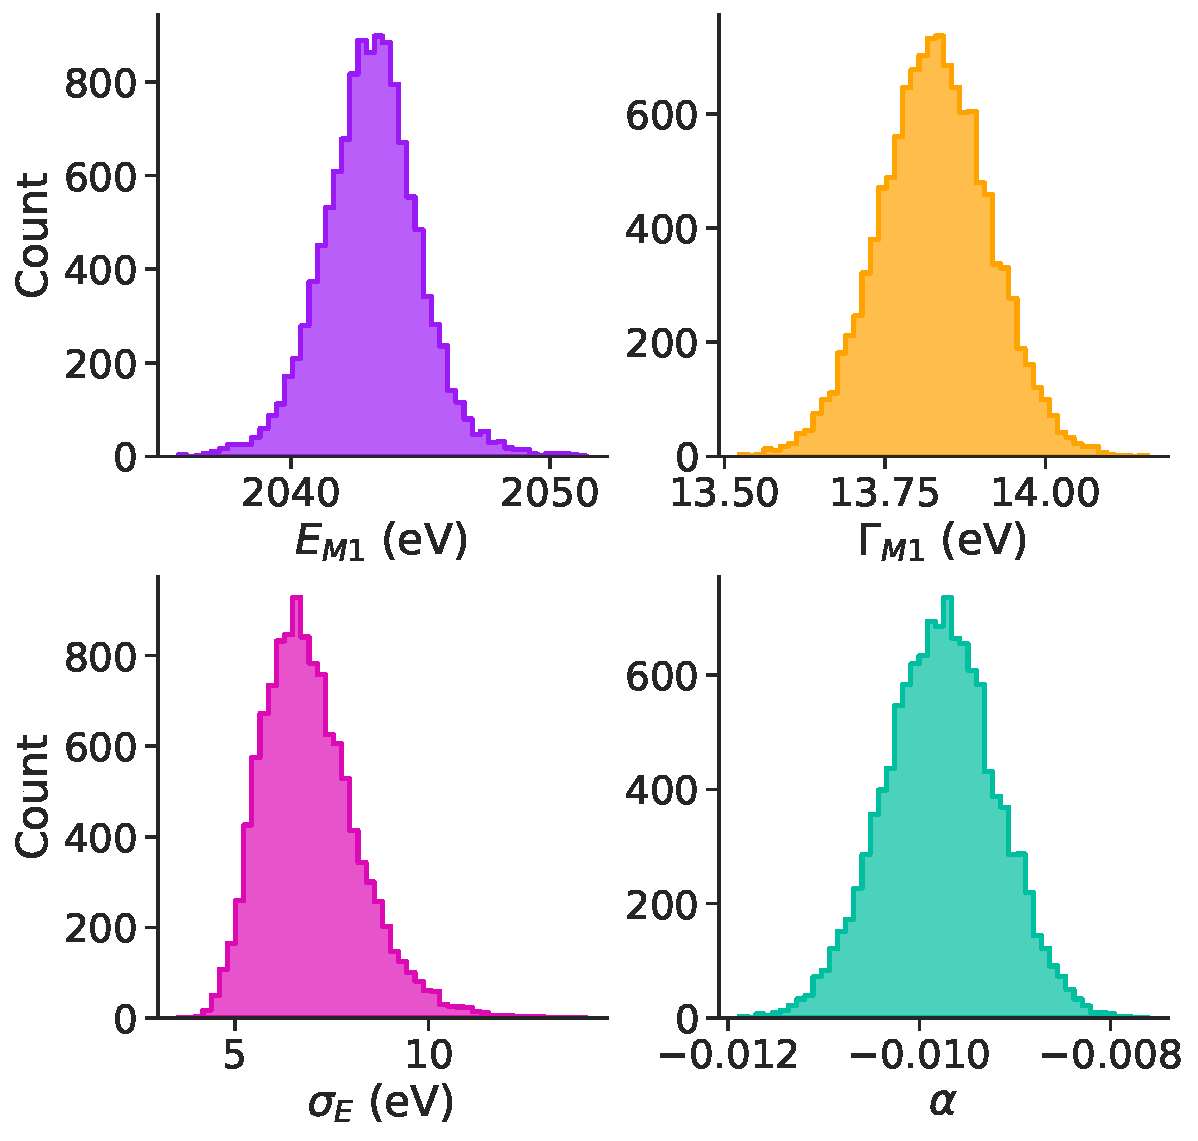
\includegraphics[width=\linewidth]{figures/ch3/peaks/dis_plot_0.pdf}
  \end{minipage}
  \hspace{0.3cm}
  \begin{minipage}{0.4\linewidth}
\begin{tabular}{lrr}
\toprule
 & Mean & StdDev \\
\midrule
  $E_{M 1}$ (eV)& 2043.1 & 1.8 \\
$\Gamma_{M 1}$ (eV)& 13.8 & 0.1 \\
$\sigma_E$ (eV)& 6.9 & 1.2 \\
$\alpha$ & $-9.8\times 10^{-3}$ & $0.6\times 10^{-3}$ \\
\bottomrule
\end{tabular}
  \end{minipage}
\caption{Results of the combined fit of 16 detectors using a hierarchical model to account for energy calibration
systematics. The posteriors of the parameters shared by all detectors are plotted on the left, while the table on the
right contains their means and standard deviations.}
\label{fig:preliminaryres}
\end{figure}
This model considers the asimmetric sigmoid lineshape without $\beta$, using $E_{M 1}$, $\Gamma_{ M 1}$, $\alpha$, $y_0$
and $m$ as global parameters to determine the true shape of the M1 peak.
Each detector is also assigned additional parameters for $\delta E$, $A$, and $FWHM$. It is assumed that each $\delta E$ follows a normal distribution around zero with a standard deviation represented by $\sigma_E$, which is the hyperparameter of the hierarchical prior.
$\sigma_E$ represents the expected spread in energy calibration among the detectors and is assigned a Gamma hyperprior centered on 8 eV, covering the range [4, 20 eV].

The likelihood is computed by iterating over the data from each detector, with the i-th detector containing a total of
$N_{tot}[i]$ events distributed across the bins. Considering that the priors of the basic model are used for the global
parameters of the peak, the new model is specified as:
\begin{eqnarray}
  \alpha &\sim& \text{normal}(0,0.15)\\
  \sigma_E &\sim& \text{gamma}(8, 1)\\
  \delta E[i] &\sim& \text{normal}(0, \sigma_E)\\
  FWHM[i] &\sim& \text{frechet}(2\times NEP[i], \;NEP[i]+0.5)\\
  A[i] &\sim& \text{normal}(1, 0.05)\\
  N_{ev}[i] &\sim& \text{poisson}(S_{\exp}(E-\delta E[i], E_{M 1}, \Gamma_{M 1}, \alpha, y_0, m, FWHM[i])\times A[i]
  \times N_{tot}[i])\qquad
\end{eqnarray}
For 16 detectors, the model contains 54 parameters and requires approximately one hour to converge and produce 500
samples from a chain, but no potential problems are identified.
Figure \ref{fig:preliminaryres} shows the posteriors of the parameters shared by all detectors, which constitute
preliminary results for the characterization of the first experimental spectrum acquired by Holmes. 
Both the obtained M1 position 2043.1$\pm 1.8$ eV and the value of $\Gamma_{M 1}=13.8\pm 0.1$ eV are consistent with other
measurements by Echo  \cite{thirdorder} within $2\sigma$ (2040 eV and 13.7 eV respectively), and differ from the first-order theoretical
predictions by some eVs as expected. 
The energy calibration dispersion in the hierarchical prior is estimated to be $\sigma_E = 6.9\pm 1.2$ eV, equivalent to the
standard deviation of the results from separate detectors. Finally, a small but nonero asimmetry is found.
Notably, the asimmetry is negative, meaning that the resonance is slightly wider at lower energies. Since the shake-off
necessarily favors higher energies, the observed asimmetry is probably due to the presence of higher-order peaks in the
M1 profile, with $E<E_{M 1}$, which have not been modeled by using a single Lorentzian.


Figure \ref{fig:systvsM1} compares the posteriors of all $\delta E$ found by the hierarchical model with those
for $E_{M 1}$ obtained by fitting the detectors separately. In order to show the distributions together, each $\delta E$
is shifted by the mean of $E_{M 1}$ found with the hierarchical model, which is plotted along with its 5-95\% credible
interval. As can be seen, the predictions for $\delta E$ are more uncertain than the separate estimates of $E_{M 1}$.
This is due to the fact that they are correlated with the global $E_{M 1}$ in the fit, and their variability reflects
that of the posterior for $E_{M 1}$. However, while the parameters of the single detectors are more uncertain in the
hierarchical model than in the separate fits, in the first all of them concurr to infer the values of the global parameters more precisely, resulting in a better estimate of
$E_{M 1}$ than the one given by the average and standard deviation of the means from separate fits $E_{M1}^{\text{sep}}=2043.2\pm
6.2$ eV.

\begin{figure}[t]
  \centering
  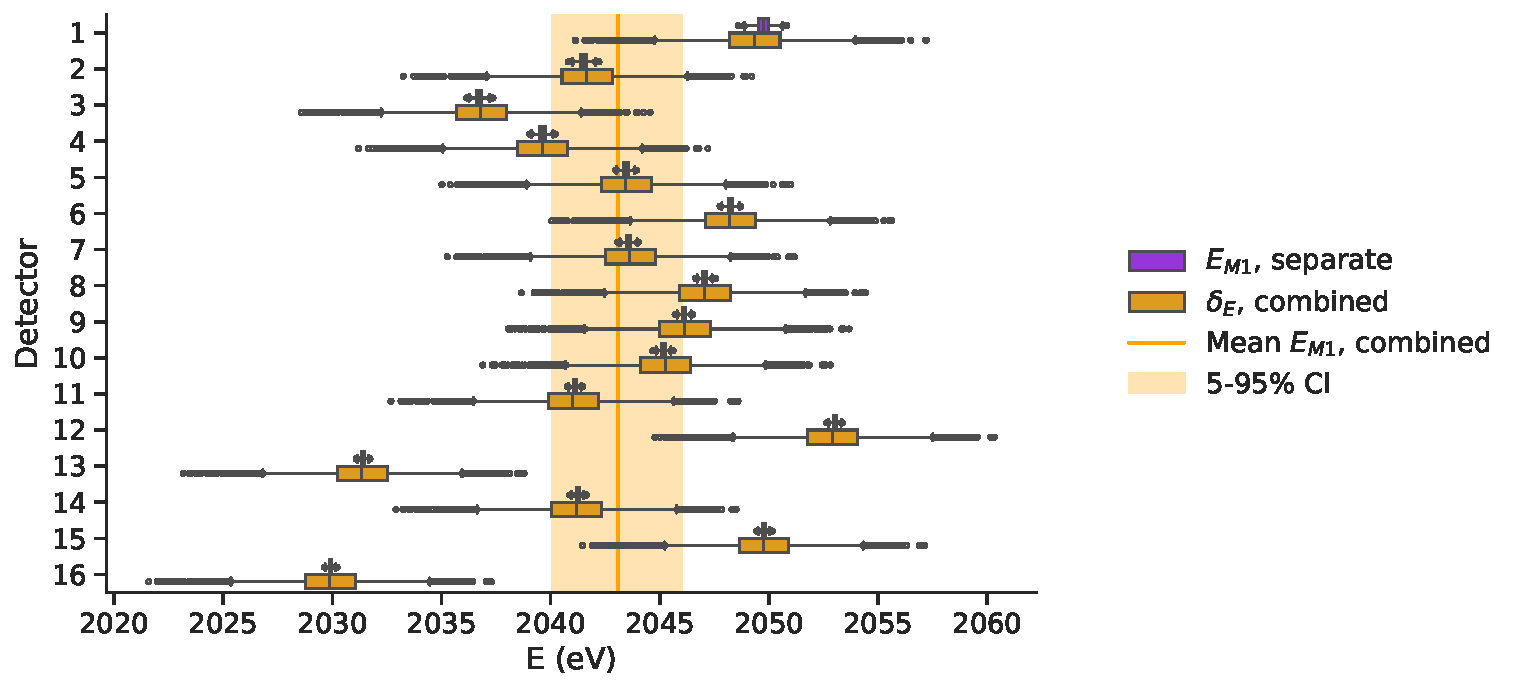
\includegraphics[width=0.9\textwidth]{figures/ch3/peaks/compare_0.pdf}
  \caption{Comparison between separate fits of the data from 16 detector and a single fit of a hierarchical model
  considering the energy sistematics $\delta E$.}
  \label{fig:systvsM1}
\end{figure}

\section{Expected neutrino mass limit}

\subsection{Data generation}

The current experimental data doesn't allow to provide a meaningful limit on the neutrino mass, since all completed and
processed measurements so far used calibration sources that obscure the endpoint region. This section of the thesis
aims to estimate the upper limit on the electronic neutrino mass achievable by Holmes in the near future using its current setup and an array implanted with a low dose of $^{163}$Ho. 
In Bayesian data analysis, the upper limit of a parameter is determined by the quantile of its posterior corresponding
to a certain credibility $\alpha$. Because of this, the limit $m_{\text{lim}}$ for $m_\nu$ will be calculated as:
\begin{equation}
\int_0^{m_{\text{lim}}} dm_\nu p(m_\nu\mid y) = 1-\alpha
\end{equation}
where $p(m_\nu\mid y)$ represents the marginal posterior of $m_\nu$.

To simulate the results of a measurement campaign, fake energy spectrum data are generated using Monte Carlo simulation
and then fitted. Since the shape of the endpoint doesn't appear to strongly depend on the rest of the spectrum, which
will be thoroughly characterized in the upcoming measurements of Holmes, the simulated dataset is generated
considering as a theoretical model the first-order spectrum. Finite energy resolution, background, and pile-up are then added.


Starting from the first-order spectrum $S(E)$ with fixed parameters, the experimental spectrum used for data generation
and fitting is given by:

\begin{equation}
S_{\text{exp}}(E) = [(1-f_{\text{pp}}-f_{\text{bkg}})S(E) + f_{\text{pp}} S(E) * S(E)+ f_{\text{bkg}}] * \text{Normal}(0, \text{FWHM})
\end{equation}

This spectrum is then binned and normalized in the ROI. A new dataset is generated by fluctuating the spectrum according to Poisson statistics, with a rate of $S_{\text{exp}}(E)\times A_{Ho}\times N_{\text{days}}$ in every bin. 
\begin{figure}
  \begin{minipage}{0.55\linewidth}
    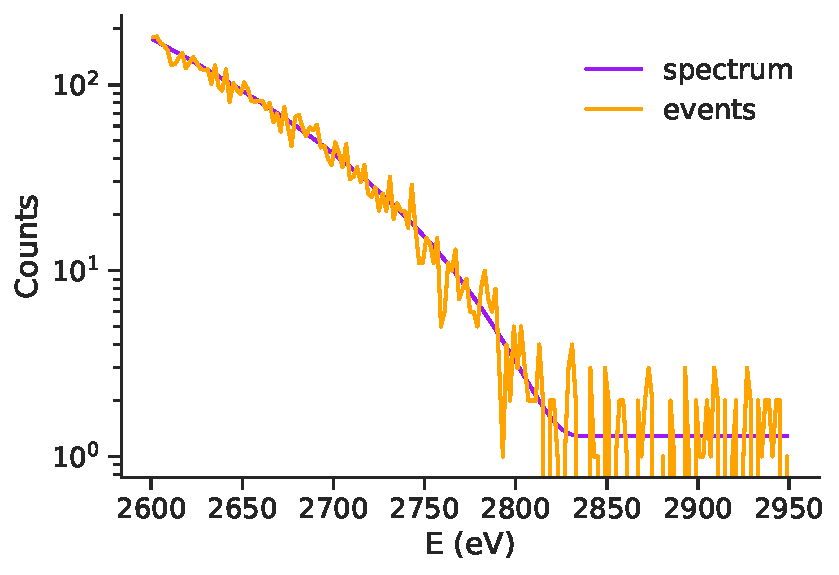
\includegraphics[width=\linewidth]{figures/ch3/endpoint/generated_0.pdf}
  \end{minipage}
  \hfill
  \centering
  \begin{minipage}{0.4\linewidth}
    \begin{tabular}{l r} \hline 
      \toprule
         Parameter & Value\\
         \midrule
         $m_\nu$& 0 eV\\
         Q& 2833 eV\\
         $A_{Ho}$& 1 Bq\\ 
         $N_{days}$& 100\\
         $N_{det}$& 64\\
         $FWHM$& 7 eV\\
         ROI& 2600-2950 eV\\ 
         \bottomrule
    \end{tabular}
  \end{minipage}
\caption{Example of simulated spectrum combining the observations of 64 identical detectors. The table shows the
parameters used for the simulation.}
\label{fig:simdata}
\end{figure}

This analysis will focus on a possible near-term measurement campaign with a baseline of 64 detectors implanted with $A_{Ho}\sim1$ Bq each, resulting in approximately 5900 events in the ROI, defined to be between 2600 eV and 2950 eV. An example of simulated data and the corresponding parameters are shown in Fig \ref{fig:simdata}.


According to the estimates of Sec \ref{sec:expected}, the expected fraction of background events in the ROI
due to radioactivity and cosmic rays is $f_{\text{bkg}}\sim 3\%$, while the pileup fraction is $f_{\text{pp}}\sim
5\times 10^{-4}$. The pileup spectrum in the ROI only weakly depends on $Q$ and $m$, which are the main free parameters
in this analysis. Furthermore, the flat background is more than 15 times higher than the pileup at every point in the
ROI, and the available statistics do not allow to differentiate between the two, since approximately 2.5 pileup events
are expected in the whole measurement. Therefore, the background will be approximated with a prevalent flat component
summed to a fixed pileup generated from the first-order spectrum, with $f_{\text{pp}}$ set to its expected value.

\subsection{Single detector}

This section discusses the basic model used for analyzing data in the endpoint region. The simulated data assumes that
all the detectors are identical, combining all the observations into a single experimental spectrum as if it originated
from one detector with the compound statistic. 


The model involves five parameters: $m_{\nu}$, $Q$, the fraction of flat background $f_{bkg}$, the energy resolution
$FWHM$, and a normalization factor $A$.
To assess Holmes' sensitivity to $m_{\nu}$, a flat prior ranging from 0 to $m_{max}=$ 300 eV is assigned to $m_{\nu}$.
This constraint ensures that the mass remains positive, while values greater than $m_{max}$ would cause the spectrum
endpoint to fall outside the ROI, rendering inference impossible.
On the other hand, the other parameters can be given more informative priors, since they model the systematics involved
in the experiment. The prior for $Q$ is a gaussian centered on the value obtained with a Penning trap measurement
$Q=2833\pm 30^{stat}\pm 15^{syst}$  \cite{eliseev2015direct}, assuming to
combine the statistic and systematic errors in quadrature. The prior for $f_{bkg}$ is a
Beta distribution with mean $0.06$ and extending between  $0$ and  $0.2$, covering the expected background fraction. The
prior for $FHWM$ is a gaussian with mean and standard deviation corresponding to those of the detectors measured in the
previous section, while $A$ is considered to be normally distributed around 1 with variation  $\pm 5\%$.
The complete model specification is given by:
\begin{eqnarray}
  m_{\nu}&\sim& \text{uniform}(0, 300)\\
  Q &\sim& \text{normal}(2833, 33.5)\\
f_{bkg}&\sim& \text{beta}(1.2,20)\\
FWHM & \sim & \text{normal}(7, 1.2)\\
A &\sim& \text{normal}(1, 0.05)\\
N_{ev} &\sim& \text{poisson}(S_{exp}(E, m_{\nu}, Q, f_{bkg}, FWHM)\times A \times N_{tot})
\end{eqnarray}
Where $N_{tot}$ is the total number of events. The implementation of the model in Stan procedes in the same way as for
the lorenztian peaks, using FFTs to compute the convolution of the binned spectrum with the gaussian energy response.
The posterior predictive check and posterior distributions for the parameters are shown in Fig \ref{fig:endcorr}. 
\begin{figure}[t]
\begin{subfigure}[b]{0.45\linewidth}
    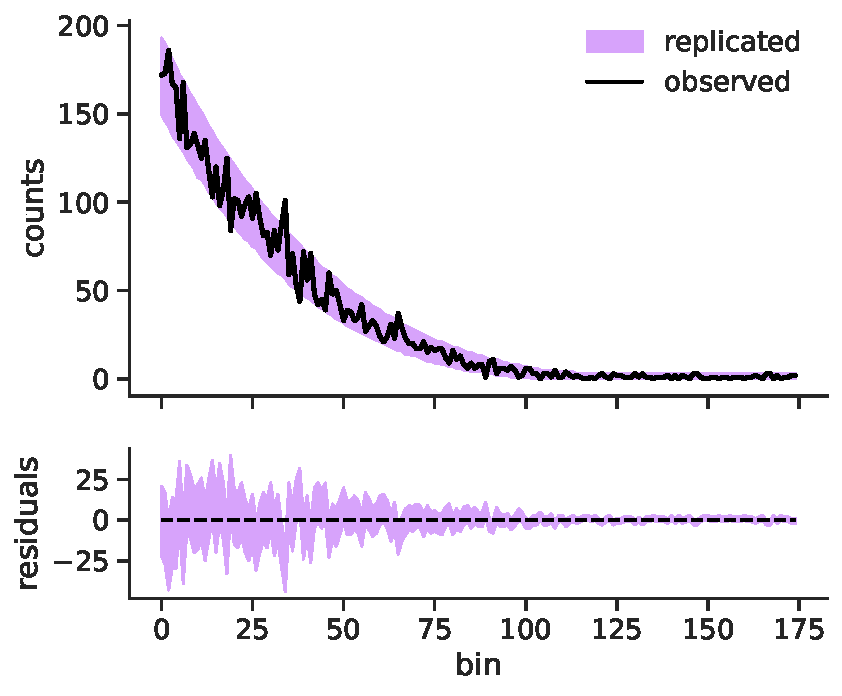
\includegraphics[width=\linewidth]{figures/ch3/endpoint/predictive_check_1.pdf}
\caption{}
\end{subfigure}
\hfill
    \begin{subfigure}[b]{0.54\linewidth}
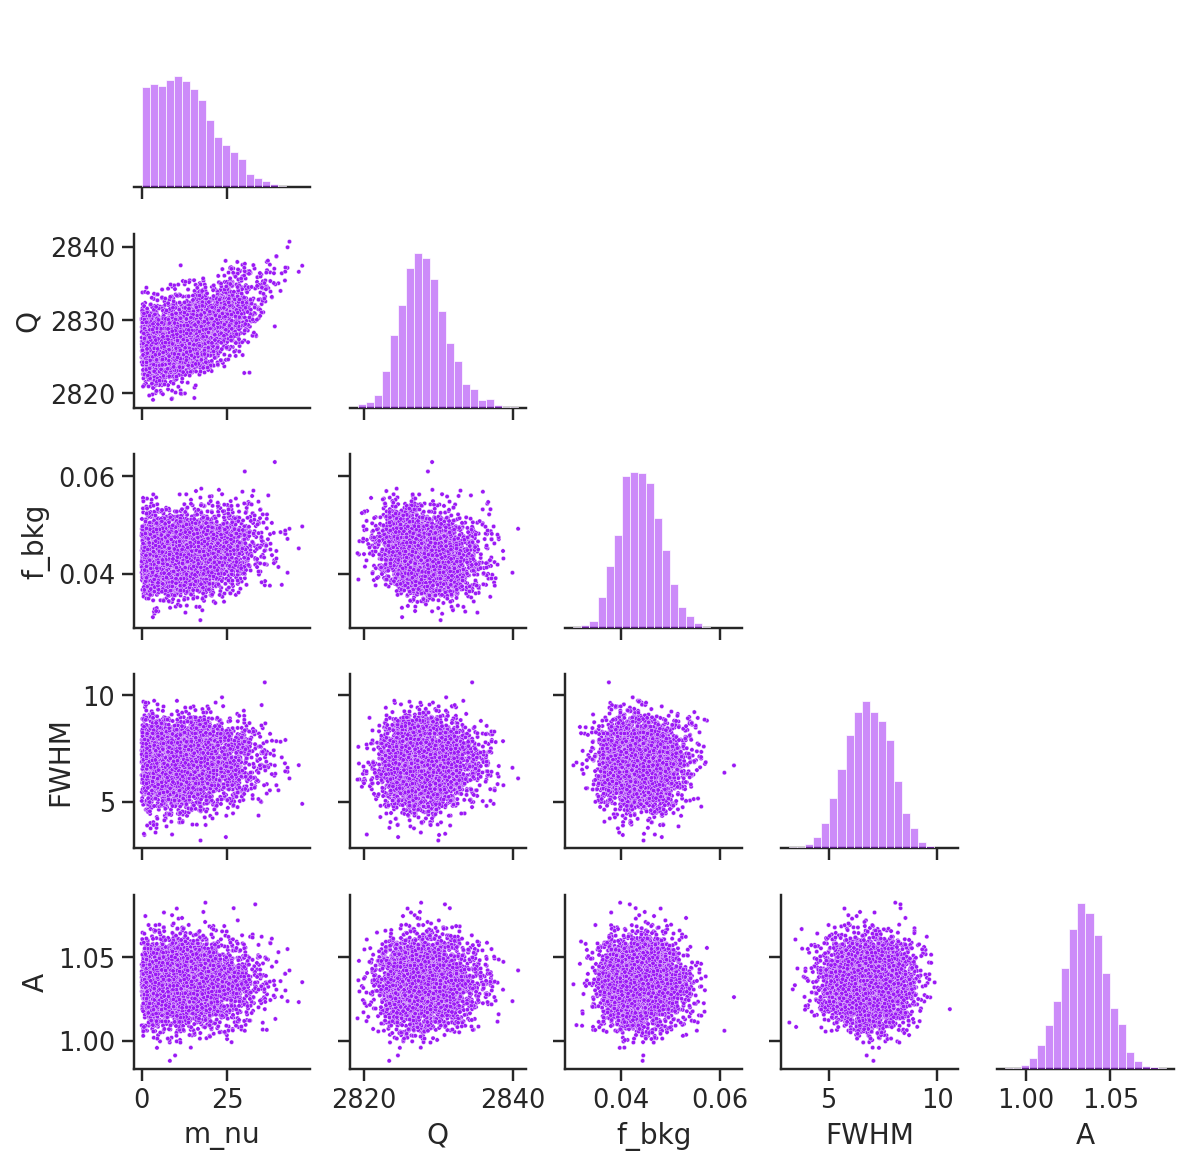
\includegraphics[width=\linewidth]{figures/ch3/endpoint/pair_grid_0.png}
\caption{}
\end{subfigure}
\caption{Posterior predictive check for the simple endpoint model (a). Correlations between parameters in the posterior of
the model (b).} 
\label{fig:endcorr}
\end{figure}

This model typically requires less than two minutes to generate a chain with around 1000 samples. It can be employed to explore the fundamental interactions between the parameters and assess its robustness in tasks requiring many iterations, such as sensitivity analysis and simulation-based calibration, before extending its scope.

The most notable correlation arises between $m_\nu$ and $Q$, since both parameters determine the endpoint.
 Moreover, the correlation induces a curve that terminates in a sharp corner. Since an
alternative parametrization that uncorrelates $m_\nu$ and $Q$ is difficult to obtain due to the
phase space formula, in this case an informative prior on $Q$ is required not only to otain better inference on  $m_\nu$ but
to avoid divergent transitions. Ideally, part of the measurement could be used to estimate $Q$ better than the value in
the literature and use the result as a more stringent prior. 
Preliminary results from Echo's high-statistics measurements suggest a new estimate of $Q=2837\pm 5^{\text{stat}}\pm
5^{syst}$ eV  \cite{velte2020measurement}. However, using this new value as a prior doesn't appear to significantly alter
the posterior of $m_\nu$.

Another less apparent but important correlation in Fig \ref{fig:endcorr} is the one between $Q$ and  $f_{bkg}$. Being negative, this
correlation hints at the fact that higher background rates limit the ability to accurately measure $Q$ and consequently
$m_\nu$ by covering the
endpoint. However, measuring how
the sensitivity of Holmes changes relative to different overall values of the systematics is beyond the scope of this analysis, which is focused on prior sensitivity. For the latter, the inference on $f_{bkg}$ is robust, allowing to recover the
simulated value of $f_{bkg}$ as long as the priors constrain it to be $<0.2$.

\begin{figure}[t]
\begin{subfigure}[b]{0.5\linewidth}
    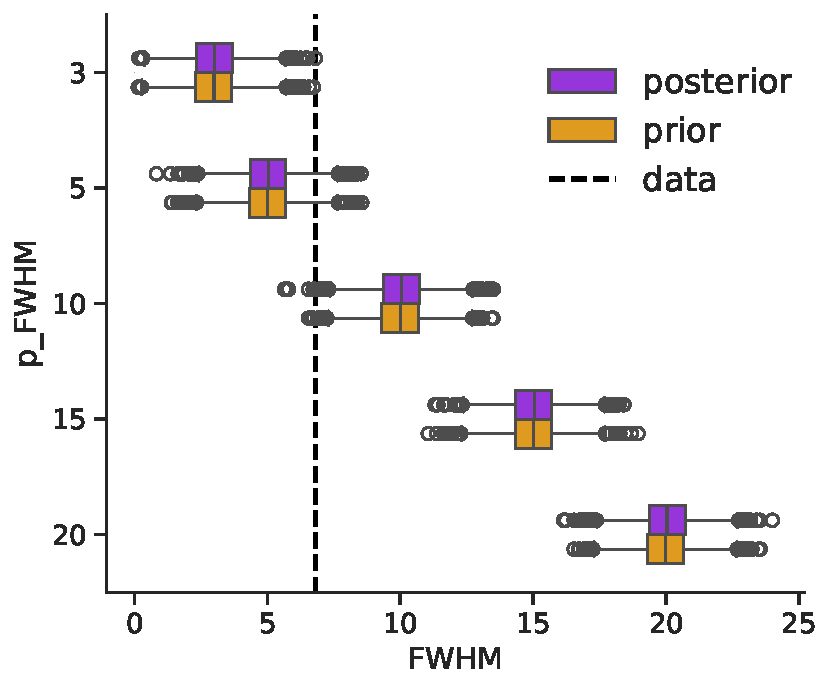
\includegraphics[width=\linewidth]{figures/ch3/endpoint/sensitivity_FW_0.pdf}
\caption{}
\end{subfigure}
%\hfill
    \begin{subfigure}[b]{0.5\linewidth}
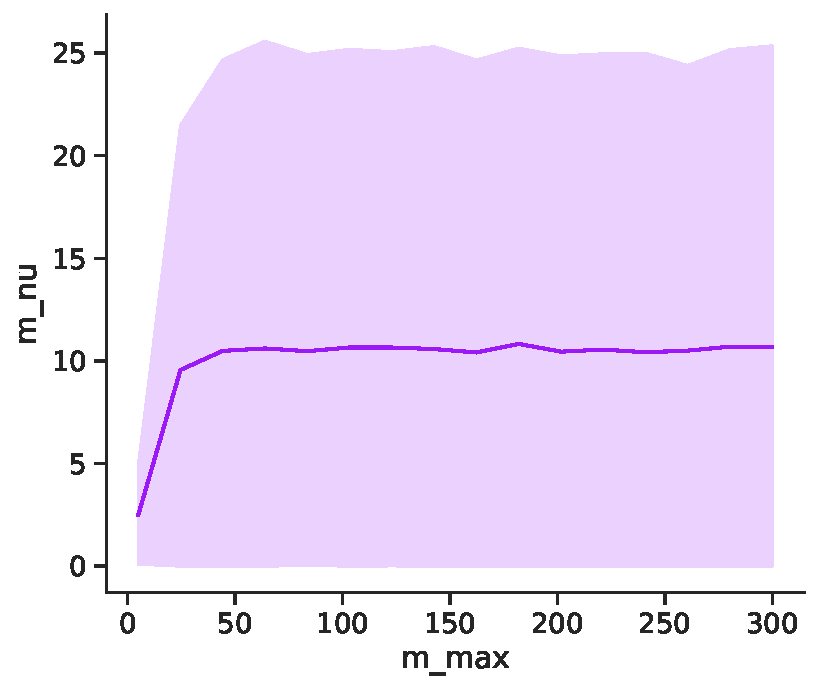
\includegraphics[width=\linewidth]{figures/ch3/endpoint/sensitivity_0.pdf}
\caption{}
\end{subfigure}
\caption{Results of sensitivity analysis of the simple endpoint model. The experimental resolution doesn't seem to affect
the fit procedure, always resulting in equal priors and posterior for data generated with a fixed $FWHM=7$ eV (a).
Posterior 95\% HDI and median for $m_\nu$ as a function of its prior maximum value $m_{max}$. Values of $m_{max}$ higher
than the relevant scale of the posterior ($\sim 50$ eV) do not affect inference.} 
\label{fig:endsensitivity}
\end{figure}
To investigate whether the problematic correlation between $m_\nu$ and $Q$ introduces biases in the posterior estimation,
the performance of HMC in fitting this model is assessed using Simulation-Based-Calibration.
The results indicate that Stan can correctly sample from the posterior.% However, it's essential to adjust the region of
%interest depending on the simulated value of $m_\nu$ to center it around the endpoint.

Interestingly, when fitting this model, the energy resolution ($FWHM$) does not seem to substantially influence the
results based on the available statistics. There appears to be little information about $FWHM$ that can be extracted
from the data when focusing solely on the ROI. Sensitivity analysis involving resolutions between 1-20 eV reveals that
the posterior for $FWHM$ is essentially the same as its prior distribution, regardless of the true value used to
generate the data (Figure 2a). Moreover, the upper limit on $m_\nu$ remains relatively constant even when considering
prior values of $FWHM$ both higher and lower than that used in data generation. The upper limit on $m_\nu$ only begins to worsen with grossly misspecified priors (e.g., $FWHM_{prior}>20$ eV for data with $FWHM=7$ eV).
Therefore, the $FWHM$ can be constrained with a narrow prior obtained from peak fitting or the NEP estimate, but it
could also be set to a fixed estimate to simplify the model.

Another interesting factor to be tested with sensitivity analysis is the robustness of the posterior of $m_{\nu}$ to the upper
limit of its prior, denoted as $m_{max}$. In fact, some practitioners advise against using flat priors, even when
defined over a finte range, since the posterior can become very dependent to the prior's limits due to the
discontinuities at the edges. This is not the case for this model, as shown in Fig \ref{fig:endsensitivity} (b), where the
posterior of $m_\nu$ doesn't seem to be influenced from the prior after $m_{max}>50$ eV.%, as would be expected from the 90\%

%\begin{figure}[h]
%    \begin{subfigure}[b]{0.24\linewidth}
%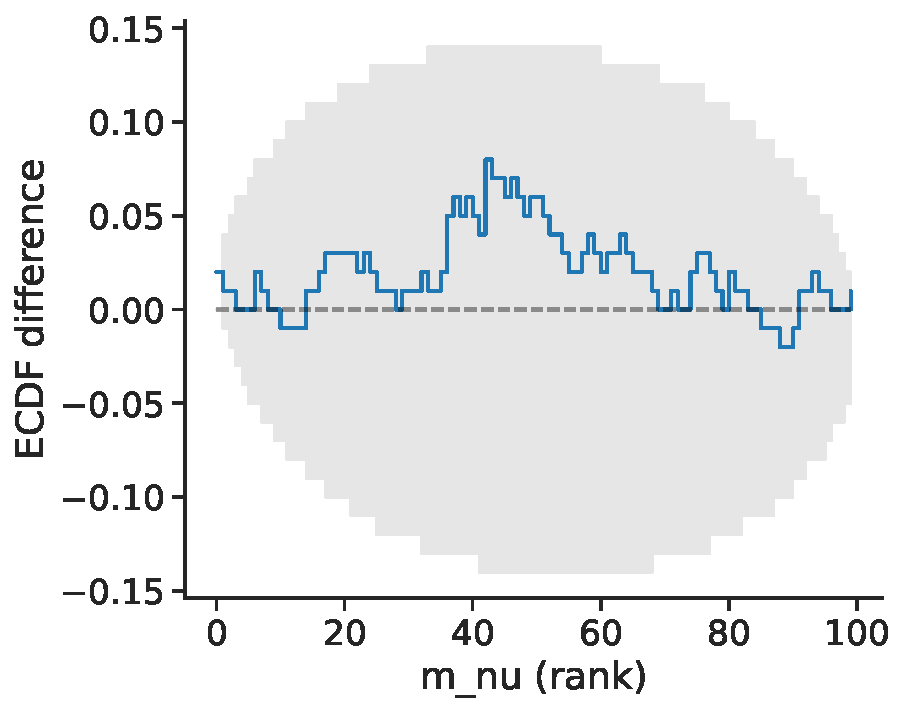
\includegraphics[width=\linewidth]{figures/ch3/endpoint/SBC_0.pdf}
%\end{subfigure}
%\begin{subfigure}[b]{0.24\linewidth}
%    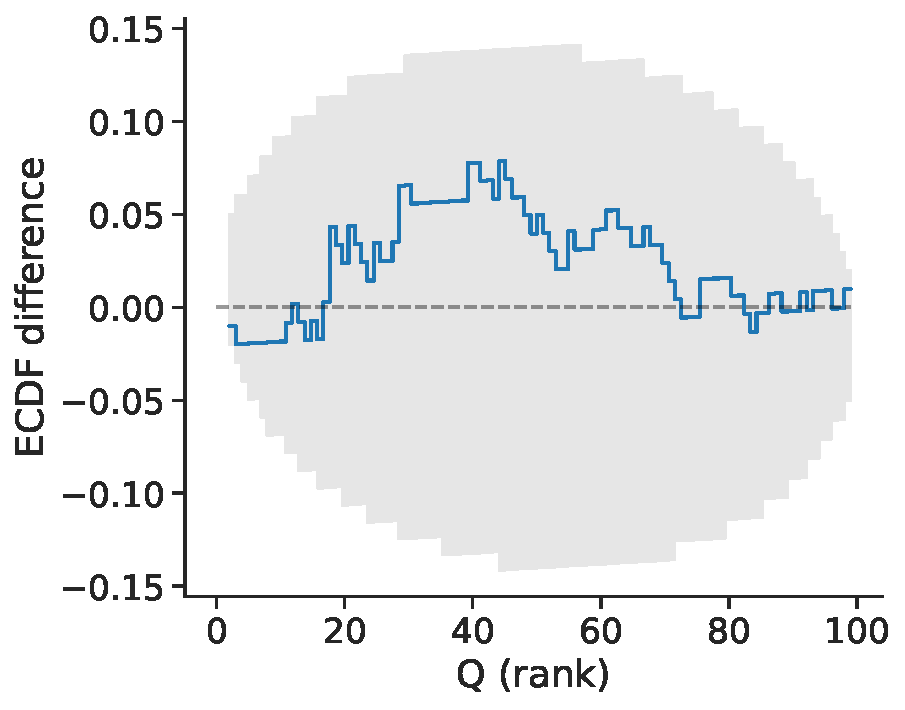
\includegraphics[width=\linewidth]{figures/ch3/endpoint/SBC_1.pdf}
%\end{subfigure}
%\label{}
%    \begin{subfigure}[b]{0.24\linewidth}
%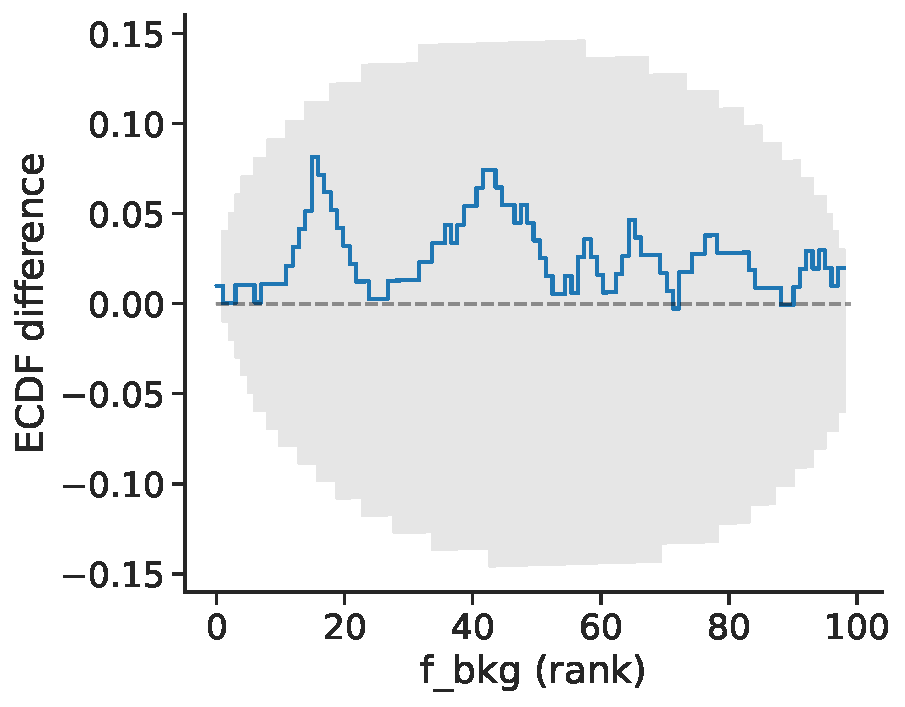
\includegraphics[width=\linewidth]{figures/ch3/endpoint/SBC_2.pdf}
%\end{subfigure}
%\begin{subfigure}[b]{0.24\linewidth}
%    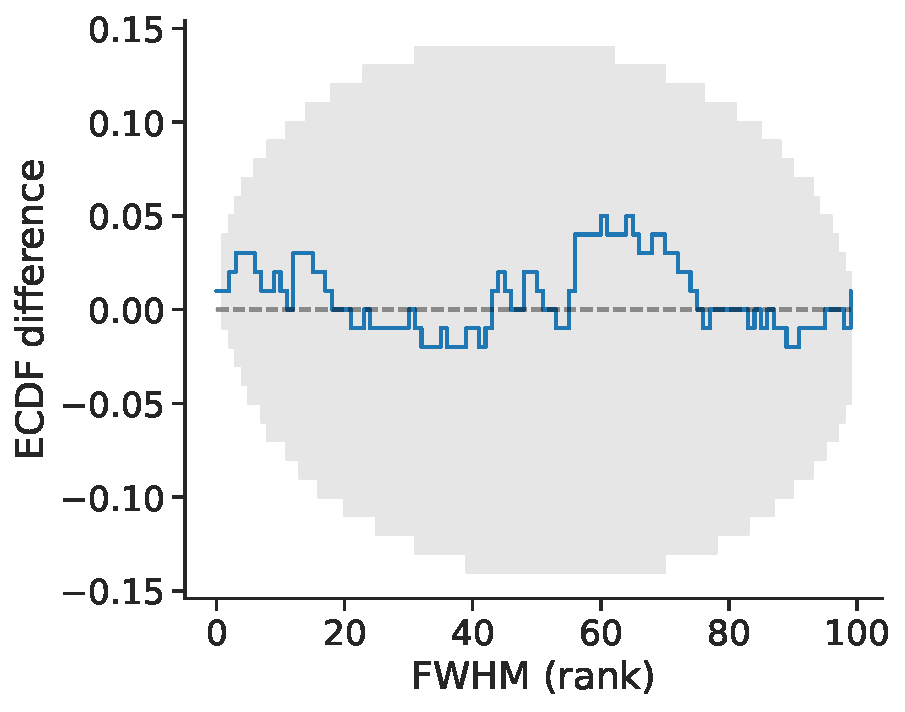
\includegraphics[width=\linewidth]{figures/ch3/endpoint/SBC_3.pdf}
%\end{subfigure}
%\caption{Results of SBC for the simple endpoint model, shown as the ECDF of the ranks for each variable.}
%\label{fig:endSBC}
%
%\end{figure}

\subsection{Deriving a robust limit}


By repeatedly fitting datasets generated with the same parameters, it becomes apparent that the
resulting posterior distributions can vary (Fig \ref{fig:endmany}). These variations cannot be attributed to the initial
Markov Chain starting point, the random number generator of the Markov Chain, or instability due to extreme sensitivity
to a prior. Instead, they seem to arise from inherent fluctuations within the data. This can be explained by the fact
that for the low overall number of collected events it is possible to obtain data with less counts than expected
exactly at the endpoint, appearing as if the neutrino mass were significantly different from zero. These fluctuations
are quite rare, appearing only in one simulation every 20, but they still present a source of additional uncertainty in
predictions based on simulated data.
\begin{figure}[b]
  \centering
  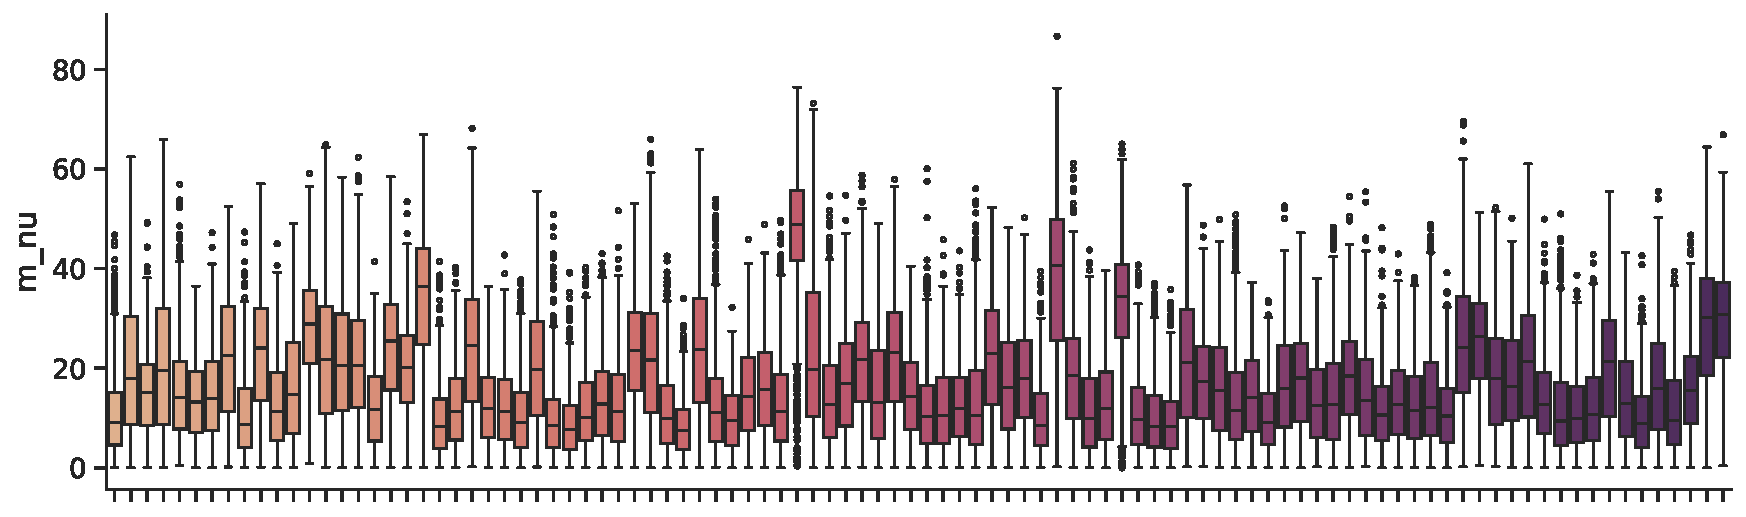
\includegraphics[width=0.8\textwidth]{figures/ch3/endpoint/cat_plot_0.pdf}
  \caption{Boxplots of 100 posteriors for $m_{\nu}$, each obtained from data simulated with the same parameters.}
  \label{fig:endmany}
\end{figure}

In cases where these fluctuations are significative, it becomes important to account for them to derive a "robust"
posterior upper limit. A straightforward approach to address this phenomenon involves simply combining the samples from
posteriors computed over different simulated datasets. While combining samples from distinct posteriors is generally
discouraged, this situation permits it due to the data being simulated from the same underlying function, and the fitting procedure's demonstrated robustness under various configurations.

It's important to clarify that this procedure does not aim to merge information from the posteriors to perform a
knowledge update, which would yield stronger limits. Rather, its purpose is to allow for additional statistical variation, resulting in a more conservative limit.

Research has shown that simply combining samples into an overall posterior and computing a single limit or interval
yields a better estimate compared to computing limits for each posterior and averaging them, which instead can
introduce bias. This concept has been demonstrated in models involving missing data  \cite{zhou2010note}, in which the missing data are
filled in by simulating from the model itself.

In this instance, it is possible to consider the analysis of simulated data as the limit case in which the data is entirely missing, but a
well-defined model exists for generating them. The main problem of this method is the necessity to  simulate data and compute the
posteriors multiple times to achieve unbiased estimates when combining the samples. To mitigate bias, around 100
iterations are required.
Figure \ref{fig:robust} shows the accumulated histogram of the 100 posteriors for $m_\nu$ plotted in Fig \ref{fig:endmany}, along with
the resulting expected limit for different credibilities.
\begin{figure}[t]
  \begin{minipage}{0.45\linewidth}
  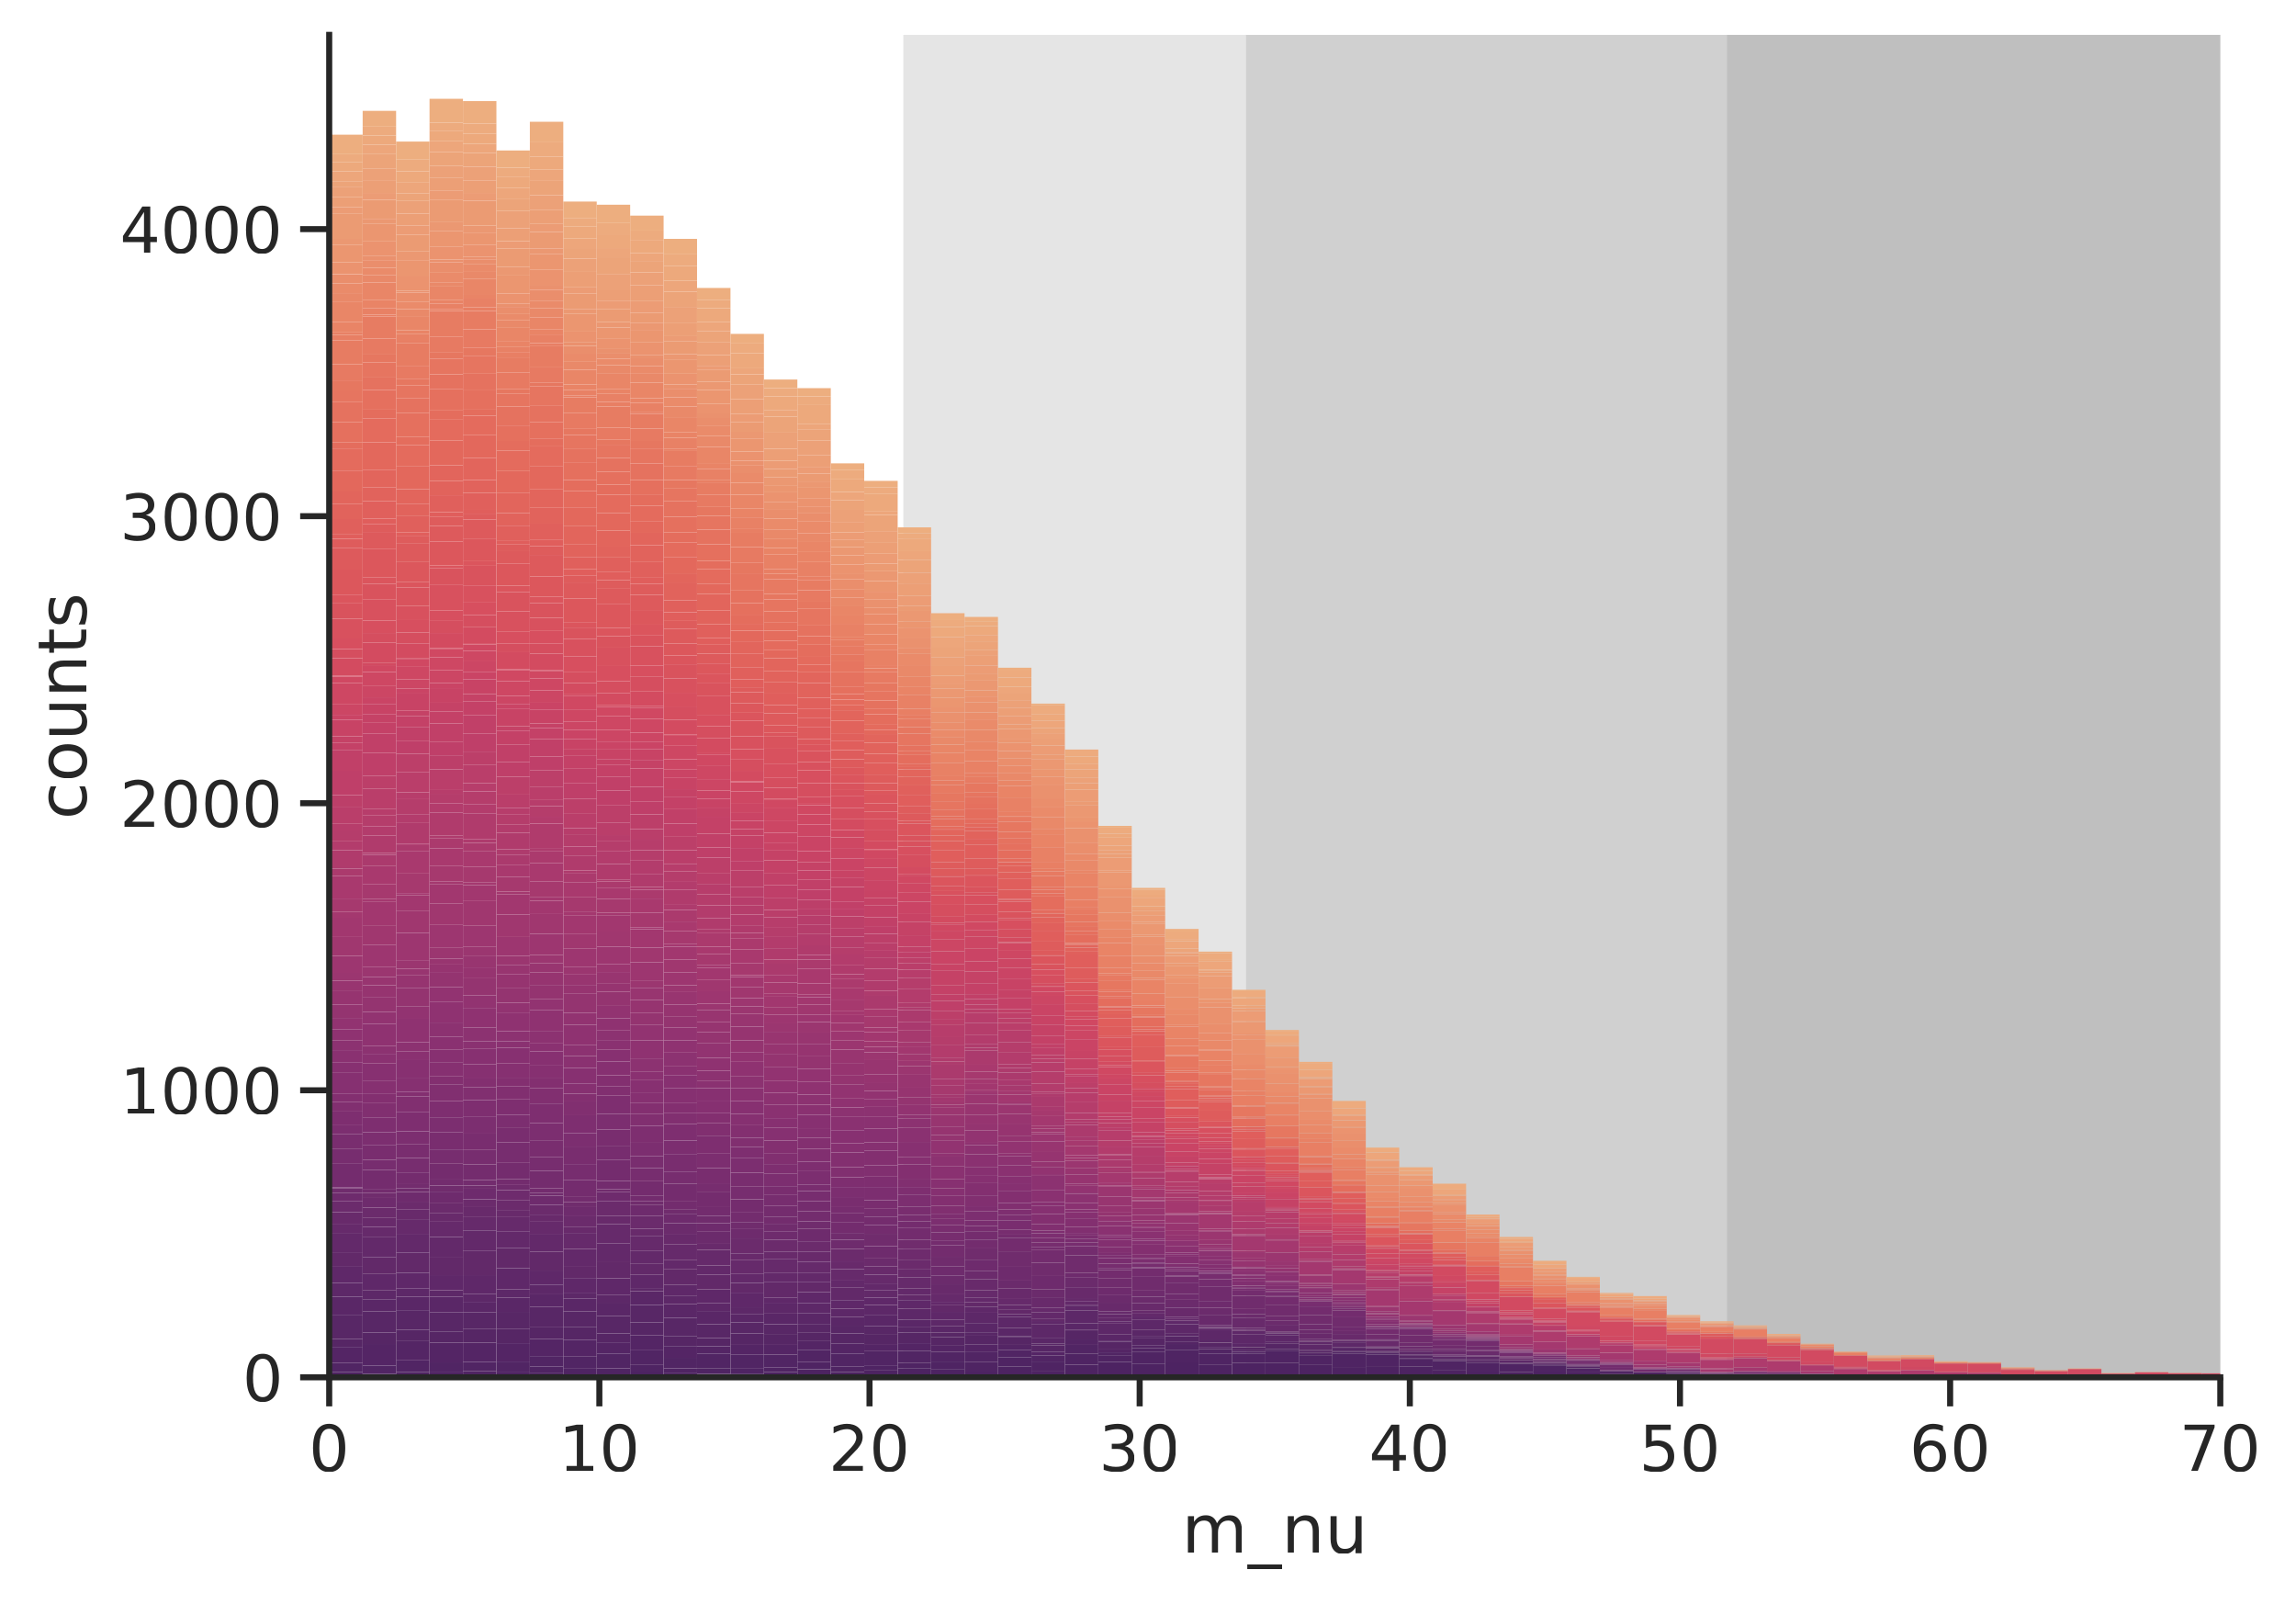
\includegraphics[width=\textwidth]{figures/ch3/endpoint/robust_0.png}
  \end{minipage}
  \hfill
  \begin{minipage}{0.45\linewidth}
    \centering
\begin{tabular}{lc}
\toprule
Credibility (\%) & $m_{\nu}$ limit (eV) \\
\midrule
68 & 21.3 \\
90  & 33.9 \\
99  & 51.7 \\
\bottomrule
\end{tabular}
\end{minipage}
\caption{Robust posterior for $m_\nu$ obtained by accumulating samples from 100 posteriors computed from data generated with fixed
parameters, considering 64 identical detectors and 100 measurement days. The table shows the resulting upper limits on
$m_\nu$ for different credibilities.}
\label{fig:robust}
\end{figure}


\subsection{Multiple detectors}
A central aspect of the data analysis for Holmes is the fact that the data is collected by many detectors, each with different characteristics and contributing with a small amount of counts in the endpoint. 
To account for this additional variation, a more realistic dataset is simulated by considering 64 detetctors with different activity, resolution and energy
systematics. For each detector, the data is generated from random values of these three quantities extracted according
to normal distributions. A gaussian spread of 0.3 is considered for the activity, while the FWHM of each detector is
distributed considering the mean and standard deviation of the resolutions observed in the characterization of the M1
peak. The energy calibration systematic is also represented by an ovreall energy shift $\delta E$ over the whole
spectrum, which is generated with mean 0 and standard deviation $8$ eV, considering a possible worst case scenario with respect
to the posterior for  $\sigma_E$ found in the last section. The same flat background $\Gamma_{bkg}=1\times 10^{-4}$ eV$^{-1}$day$^{-1}
$det$^{-1}$ is used for all detectors, resulting in different $f_{bkg}$ values due to the varying activity. The same
is done for the pileup, which is obtained considering the activity in each detector. 

The resulting dataset consists of 64 separate endpoint spectra, each containing between 50 and 150 events. 
Intuitively, to correctly account for all the information available it is necessary to model each detector separately.
In the same way as for the characterization of M1, this requires to create a single large model where the neutrino mass $m_\nu$ is used as a global parameter while some nuisance parameters $\theta_i$ describe the systematics of the i-th detector.


\begin{figure}
  \begin{minipage}{0.45\linewidth}
    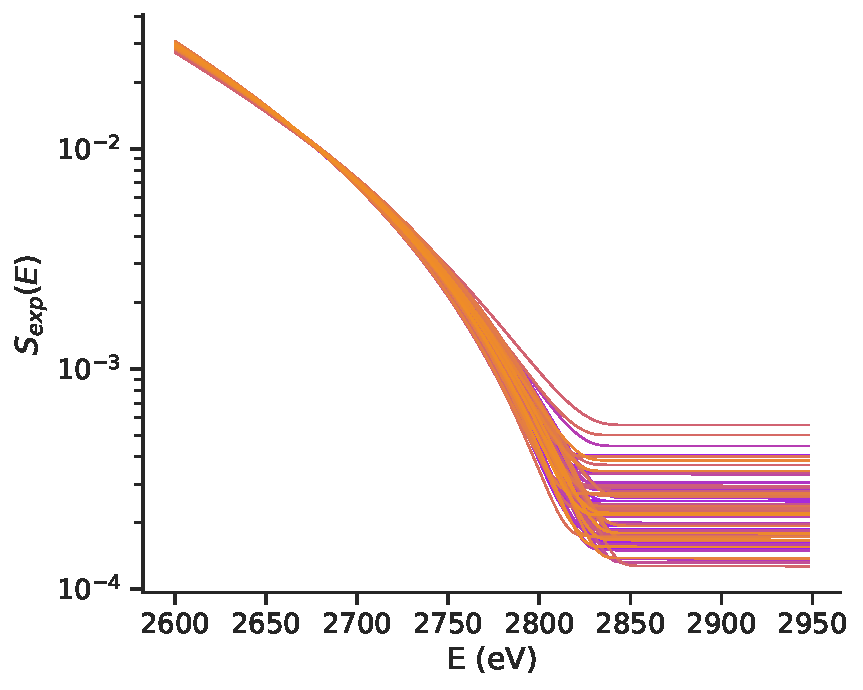
\includegraphics[width=\linewidth]{figures/ch3/endpoint/multispectrum_0.pdf}
  \end{minipage}
  \hfill
  \begin{minipage}{0.4\linewidth}
    \begin{tabular}{l r} \hline 
      \toprule
         Parameter & Value\\
         \midrule
         $m_\nu$& 0 eV\\
         Q& 2833 eV\\
         $A_{Ho}$& normal(1, 0.3) Bq\\ 
         $FWHM$& normal(7, 1.5) eV\\
         $\delta E$& normal(0, 8) eV\\
         ROI& 2600-2950 eV\\ 
         \bottomrule
    \end{tabular}
  \end{minipage}

\caption{Example of variable spectra used in the simulation of 64 different detectors, generated according to the
parameters in the table. Each spectrum is normalized in the ROI and  used to simulate between 50 and 150 events
according to the activity.}
\label{}
\end{figure}

The model previously used to fit a single spectrum is expanded in order to consider the 64 different detectors using the
same hierarchical approach as in the case of the M1 peak characterization.
Due to the computational complexity, it is necessary to use the smallest possible number of parameters to describe each detector. 
Having assessed in the previous section that, for reasonable estimates, any value of energy resolution of the detector does not
influence the estimate of $m_\nu$, and considering that the FWHM of each detector can be estimated
quite precisely from the NEP or by fitting the peak, in this model the FWHM is introduced as a constant variable.
Instead, three parameters are assigned to each detector, corresponding to the background fraction $f_{bkg}$, the energy
systematic $\delta E$ and the normalization constant $A$. Assuming that the calibration systematics are normally
distributed around 0, the corresponding parameters ${\delta E[i]}$ are grouped in a hierarchical prior with standard
deviation $\sigma_E$, which is again left as a free parameter.
The priors used in the previous analysis are assigned to $m_\nu$, $Q$ and each $f_{bkg}[i]$, while the prior on $A[i]$
is
sligthly relaxed in order to account for a larger expected variation due to a lower number of events in each detector:


\begin{eqnarray}
  m_{\nu}&\sim& \text{uniform}(0, 300)\\
  Q &\sim& \text{normal}(2833, 33.5)\\
  \sigma_E&\sim &\text{gamma}(16,2)\\
\delta E[i] & \sim & \text{normal}(0, \sigma_E)\\
f_{bkg}[i]&\sim& \text{beta}(1.2,20)\\
A[i] & \sim & \text{normal}(1, 0.15)\\
N_{ev}[i] &\sim& \text{poisson}(S(E-\delta E[i], m_{\nu}, Q, f_{bkg}[i], FWHM[i])\times A[i]\times N_{tot}[i])
\end{eqnarray}
\begin{figure}[t]
  \begin{minipage}{0.5\linewidth}
  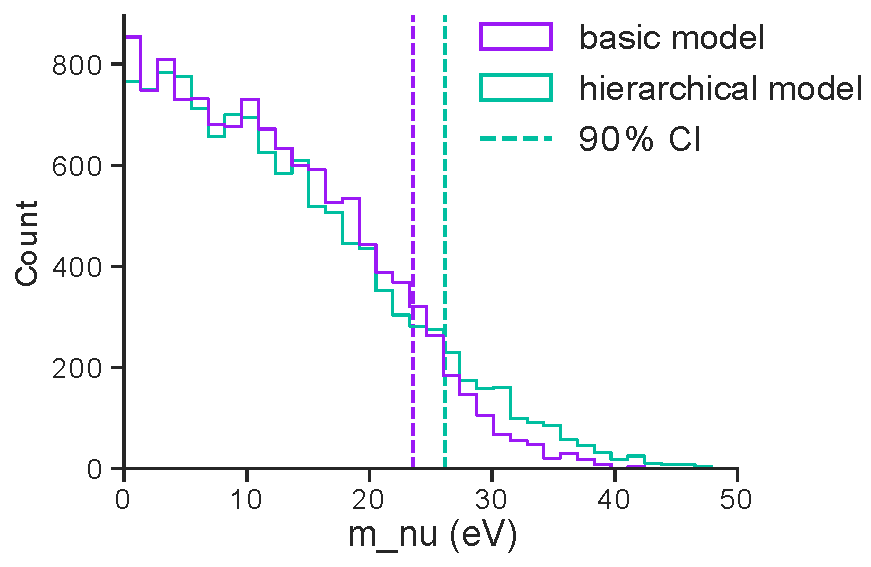
\includegraphics[width=\linewidth]{figures/ch3/endpoint/dis_plot_b_vs_h.pdf}
  \end{minipage}
  \hfill
  \begin{minipage}{0.5\linewidth}
    \centering
  \begin{tabular}{lcc}
  \toprule
%  \thead{Credibility (\%) }& \thead{$m_\nu^{lim}$ (eV) \\ identical\\ detectors} & \thead{$m_\nu^{lim}$ (eV) \\
\thead{Credibility (\%) }& \thead{$m_\nu^{lim}$ (eV) \\ hierarchical\\ model} & \thead{$m_\nu^{lim}$ (eV) \\ basic\\
model}\\
  \midrule
  68 & 16.4 & 15.7\\
  90 & 26.1 & 23.6\\
  99 & 38.2 & 33.3\\
  \bottomrule
  \end{tabular}
  \end{minipage}
\caption{Posterior distributions of $m_\nu$ for the hierarchical and basic model obtained by fitting the same simulated
  data, which considers detectors with varying systematics. The table shows the obtained upper limits on $m_\nu$ for different credibilities, with the basic model
providing lower limits.}
\label{fig:hiervsbase}
\end{figure}

The full model contains 196 parameters and requires approximately 10 hours for warm-up and generating 500 samples
from a chain. While $A$ and $f_{bkg}$ are reliably identified for each detector, and there are no divergent transitions, the
energy systematics and their hyperparameter appear less influenced by the fit. This is likely due to the extremely low
statistics available, and the inability to modify the priors introduces additional uncertainty into the posterior.
Consequently, the 90\% credibility upper limit on $m_\nu$ obtained through the hierarchical model is 3 eV worse than that achieved by combining all spectra and
fitting the compound data with the basic model, as shown in Fig \ref{fig:hiervsbase}.

The effectiveness of fitting the compound spectrum with a simple model can be attributed to the averaging out of
fluctuations in the generated data across a large number of detectors. This is especially evident given that the parameters
in the simulation follow a normal distribution. For instance, the overall effect of normally distributed $\delta E$ and $FWHM$ in each detector
appears as a broadening of the energy resolution in the combined spectrum, which can then be described by an effective
$FWHM_{eff}^2\sim\overline{FWHM}^2+FWHM_E^2$, where $FWHM_E=2\sqrt{2\ln 2}\sigma_E $ is the dispersion of the calibration
systematics. For the parameters used in the simulation $FWHM_{eff}\sim {18}$ eV, still in the range that is predicted
not to affect the upper limit on $m_\nu$ significantly in the prior sensitivity analysis of the simple model.



Since fitting the compound spectrum with the basic model is not computationally demanding, it is possible to compute a
robust limit by generating new data and repeating the analysis. This robust limit can then be compared to the one
obtained from the "perfect" spectrum generated by identical detectors, quantifying the additional uncertainty introduced
by normally varying their main systematics and using an approximate fitting procedure. The resulting two robust
posteriors and upper limits are shown in Figure \ref{fig:final}. The upper limits on $m_\nu$ are nearly identical, differing by at most 1.5 eV. Under the assumption of
normally distributed systematics among detectors and for a low-activity measurement, this demonstrates that this
simplified fitting approach can yield reasonable results without resorting to computationally expensive models. However,
it must be clarified that in an experimental setting the distribution of systematics might significantly differ from
the assumption of
normalilty, a case in which fitting the compund spectrum might not be a reasonable approximation. Furthermore,
while it might
be useful in aiding the preliminary stage of data analysis, this simplified procedure cannot subsistute
for a more thorough analysis using the hierarchical model, which could be aided by specifying more informative priors
for the systematics using additional characterization measurements.


\begin{figure}[ht]
  \begin{minipage}{0.5\linewidth}
    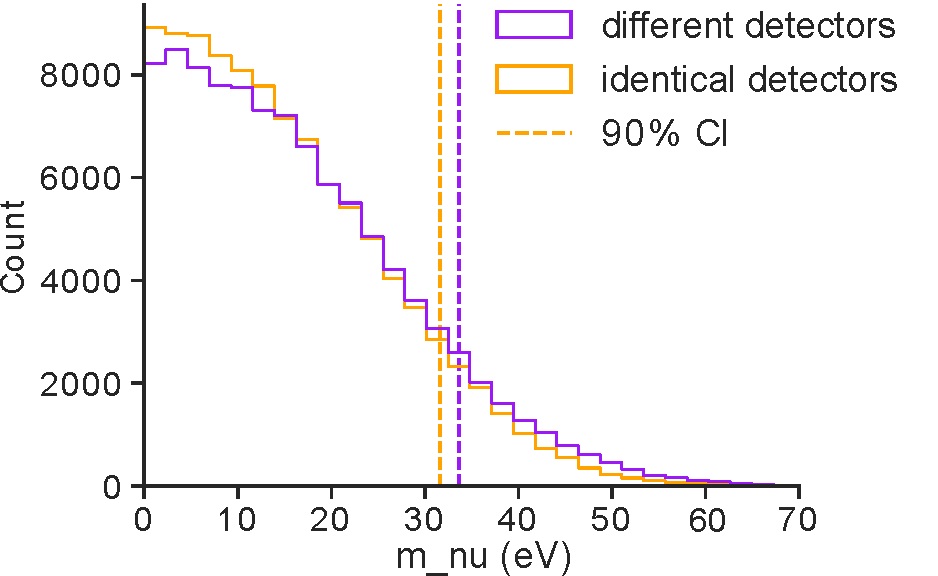
\includegraphics[width=\linewidth]{figures/ch3/endpoint/dis_plot_final.pdf}
  \end{minipage}
  \hfill
  \begin{minipage}{0.45\linewidth}
  \begin{tabular}{lcc}
   \toprule
\thead{Credibility (\%) }& \thead{$m_\nu^{lim}$ (eV) \\ identical\\ detectors} & \thead{$m_\nu^{lim}$ (eV) \\ different\\ detectors}\\
\midrule
68 & 21.3  & 21.5 \\
90 & 33.9 & 35.2 \\
99 & 51.7 & 53.1 \\
\bottomrule 
  \end{tabular}
  \end{minipage}
\caption{Robust posterior distributions of $m_\nu$ obtained with the basic model. Both results are computed from 100 simulated
datasets, comparing the robust posterior of Fig \ref{fig:robust} obtained from data considering identical
detectors (orange) with the robust posterior obtained from compound spectra of detectors with different systematics
(purple). The
resulting upper limits on $m_\nu$ are shown in the table.}
\label{fig:final}
\end{figure}
